\emph{Matrices} (singular: \emph{matrix}) are arrays of numbers, for example,
\[ M = \begin{bmatrix}
 4 & -\sqrt{3} & \pi \\ -5.2 & 0 & 13
\end{bmatrix}, \]
and \emph{vectors} are matrices that have only one column. The use of vectors and matrices makes the notation and handling of data and variables in large computations clearer and more compact, and their study has also led to new concepts and theories. Vectors and matrices are fundamental in mathematics and for applications of mathematical analysis.

In the example below, we will work with a matrix that represents the connections in a network of cities, and this matrix can therefore be considered the link that makes the road network accessible to mathematical analysis. Other networks that are frequently analysed using matrices include social networks (e.g., to study the spread of news), the world wide web (e.g., Google PageRank), contact networks (e.g., to minimise contagion in a hospital).

\begin{application}[Random walks]
A very large number of hikers is travelling randomly around the network of cities
\begin{center}
	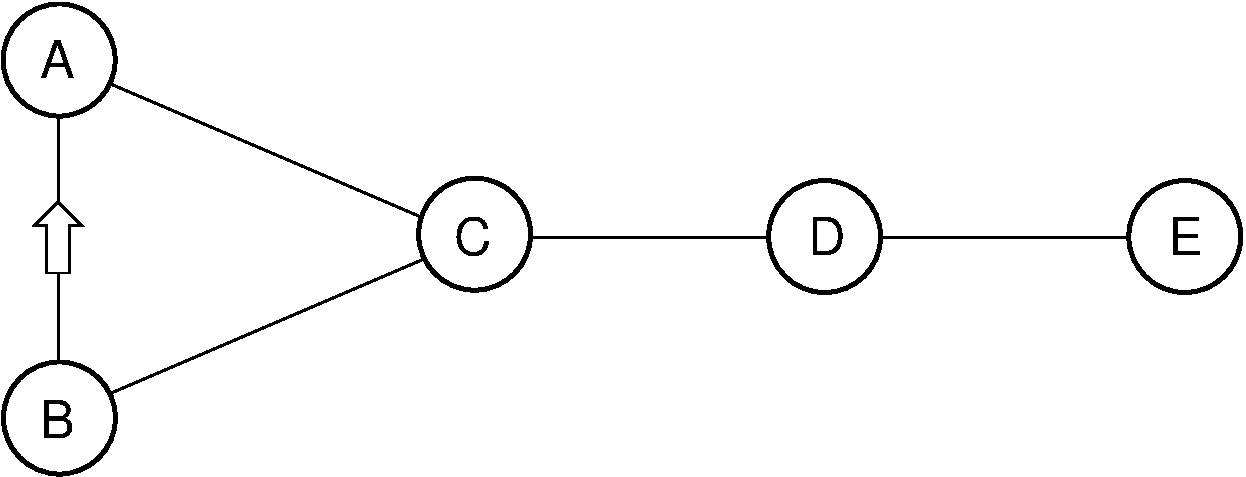
\includegraphics[width=0.5\textwidth]{./Figures/network.pdf}
\end{center}
where the road between $A$ and $B$ can only be travelled in one direction. A hiker would arrive in a city, stay for the day, randomly pick one of the outgoing roads -- each with equal probability; possibly the city he or she came from the previous day --  and then travel there the next morning. For example, if there are 100 hikers in $D$ today, then an average of 50 of them will hike to $C$ the next day. Besides those new arrivals from $D$, the city $C$ will further receive new hikers from $A$ and from $B$.

The hikers in this example are called \emph{random walkers} in mathematical jargon, and an important and applicable task is to find the \emph{steady state} of the system -- that is, the distribution of hikers so that the total number of hikers in each city does not change from one day to the next. For example, looking at the above map, you might expect that after a long time there should be a larger concentration of hikers in $C$ than in $E$.

The steady state  can be found by balancing the number of incoming and outgoing hikers for each city. Let $d$ and $e$ be the steady-state proportion of hikers in cities $D$ and $E$, and consider all travelling to and from $E$: outgoing $= e$, incoming = $\tfrac12d$, which gives $e = \tfrac12d$. Repeating this for the other cities leads to a collection of five equations.

Alternatively, one can choose a matrix approach and use vectors to describe the distribution of hikers over the network. The first entry of that vector stands for the proportion of hikers in $A$, the second for the proportion in $B$, etc. For example,
\[ v_1 = \begin{bmatrix} 0 \\ 0 \\ 1 \\ 0 \\ 0 \end{bmatrix}, \quad v_2 = \begin{bmatrix} 0.2 \\ 0.2 \\ 0.2 \\ 0.2 \\ 0.2 \end{bmatrix}\]
means in the first case that all hikers are in $C$, and in the second case that they are evenly distributed over all five cities. Next we describe their movements using a matrix. After the review of matrix multiplication in the next section, you will be able to convince yourself that
\[ v_{\text{tomorrow}} = \begin{bmatrix} 0 & \rfrac12 & \rfrac13 & 0 & 0 \\
									 0 & 0 & \rfrac13 & 0 & 0 \\
									 1 & \rfrac12 & 0 & \rfrac12 & 0 \\
									 0 & 0 & \rfrac13 & 0 & 1 \\
									 0 & 0 & 0 & \rfrac12 & 0 \end{bmatrix} v_{\text{today}}
					   = P \, v_{\text{today}} \]
reflects the movement of the hikers around the network of cities\footnote{For example:
\[ \text{all hikers in $C$} \leftrightarrow
v = \begin{bmatrix} 0 \\ 0 \\ 1 \\ 0 \\ 0 \end{bmatrix}
\quad \stackrel{P}{\longrightarrow} \quad
P \, v = \begin{bmatrix} \rfrac13 \\ \rfrac13 \\ 0 \\ \rfrac13 \\ 0 \end{bmatrix}
\leftrightarrow  \text{ hikers evenly distributed over $A,B,D$}
\qquad \text{\checkmark} \]
Now check this for the other four ``concentrated'' configurations. If that works, then $P$ is correct.
}. The task of finding a steady state now corresponds to finding a vector (i.e., a distribution of hikers) that does not change through application of $P$ (i.e., from one day to the next). Note that individual hikers keep moving -- the steady state is the distribution of hikers such that their \emph{total} number in each city stays the same. Denoting this vector by $v^*$ and its entries $a,b,c,d,e$, we obtain $v^*=Pv^*$, or
\[ \begin{bmatrix} a\\b\\c\\d\\e \end{bmatrix} =
\begin{bmatrix} 0 & \rfrac12 & \rfrac13 & 0 & 0 \\
0 & 0 & \rfrac13 & 0 & 0 \\
1 & \rfrac12 & 0 & \rfrac12 & 0 \\
0 & 0 & \rfrac13 & 0 & 1 \\
0 & 0 & 0 & \rfrac12 & 0 \end{bmatrix} \begin{bmatrix} a\\b\\c\\d\\e \end{bmatrix}. \]
This is an equation of 5-vectors (the result of the matrix multiplication on the right-hand side is a 5-vector as well) and therefore corresponds to a collection of five ordinary equations -- can you locate the equation $e = \tfrac12d$ from the previous paragraph in it?

The equation $v^*=Pv^*$ is in fact an eigenvalue equation for the matrix $P$. We will learn how to solve it in this chapter. The solution is
\[a=0.177,\:\:b=0.118,\:\:c=0.353,\:\:d=0.235,\:\:e=0.118\:.\]
\end{application}


\section{Review of Matrix Arithmetic}
\label{sec:rma}
\begin{definition}[Matrices] ~\\
\begin{enumerate}[(i)]
	\item A $m \times n$ matrix is an array
		\[A = \begin{bmatrix}
		a_{11} & a_{12} & a_{13} & \cdots & a_{1n} \\
		a_{21} & a_{22} & a_{23} & \cdots & a_{2n} \\
		a_{31} & a_{32} & a_{33} & \cdots & a_{3n} \\
		\vdots & \vdots & \vdots & \ddots & \vdots \\
		a_{m1} & a_{m2} & a_{m3} & \cdots & a_{mn} \\
		\end{bmatrix},\]
		where $m$ is the number of rows and $n$ the number of columns. We also refer to $A$ as a matrix of \emph{size} $m \times n$.
	\item An equation of the form $A=B$, where $A$ and $B$ are matrices of the same size $m \times n$, means that $a_{ij} = b_{ij}$ for all $i\in\{1,2,\dots,m\},j\in\{1,2,\dots,n\}.$ Matrices of different sizes can never be equal.
	\item Addition and subtraction can only be carried out for matrices of the same size, and then the operation is carried out elementwise:
		\begin{equation*}\begin{split}
		A \pm B & = \begin{bmatrix}
		a_{11} & a_{12} & \cdots & a_{1n} \\
		a_{21} & a_{22} & \cdots & a_{2n} \\
		\vdots & \vdots & \ddots & \vdots \\
		a_{m1} & a_{m2} & \cdots & a_{mn} \\
		\end{bmatrix} \pm \begin{bmatrix}
		b_{11} & b_{12} & \cdots & b_{1n} \\
		b_{21} & b_{22} & \cdots & b_{2n} \\
		\vdots & \vdots & \ddots & \vdots \\
		b_{m1} & b_{m2} & \cdots & b_{mn} \\
		\end{bmatrix} \\ & = \begin{bmatrix}
		a_{11} \pm b_{11} & a_{12} \pm b_{12} & \cdots & a_{1n} \pm b_{1n} \\
		a_{21} \pm b_{21} & a_{22} \pm b_{22} & \cdots & a_{2n} \pm b_{2n} \\
		\vdots & \vdots & \ddots & \vdots \\
		a_{m1} \pm b_{m1} & a_{m2} \pm b_{m2} & \cdots & a_{mn} \pm b_{mn} \\
		\end{bmatrix}.
		\end{split}\end{equation*}
	\item Multiplying a number with a matrix is called \emph{scalar multiplication}:
		\[ \lambda A = \lambda \begin{bmatrix}
		a_{11} & a_{12} & \cdots & a_{1n} \\
		a_{21} & a_{22} & \cdots & a_{2n} \\
		\vdots & \vdots & \ddots & \vdots \\
		a_{m1} & a_{m2} & \cdots & a_{mn} \\
		\end{bmatrix} = \begin{bmatrix}
		\lambda a_{11} & \lambda a_{12} & \cdots & \lambda a_{1n} \\
		\lambda a_{21} & \lambda a_{22} & \cdots & \lambda a_{2n} \\
		\vdots & \vdots & \ddots & \vdots \\
		\lambda a_{m1} & \lambda a_{m2} & \cdots & \lambda a_{mn} \\
		\end{bmatrix}.\]
	\item Multiplying two matrices $A$ and $B$ is called \emph{matrix multiplication} -- it can be carried out only if the number of columns of $A$ agrees with the number of rows of $B$:
		\begin{equation*}
		A \, B =\begin{bmatrix}
		a_{11} & a_{12} & \cdots & a_{1n} \\
		a_{21} & a_{22} & \cdots & a_{2n} \\
		\vdots & \vdots & \ddots & \vdots \\
		a_{m1} & a_{m2} & \cdots & a_{mn} \\
		\end{bmatrix} \begin{bmatrix}
		b_{11} & b_{12} & \cdots & b_{1k} \\
		b_{21} & b_{22} & \cdots & b_{2k} \\
		\vdots & \vdots & \ddots & \vdots \\
		b_{n1} & b_{n2} & \cdots & b_{nk} \\
		\end{bmatrix}
		= \begin{bmatrix}
		c_{11} & c_{12} & \cdots & c_{1k} \\
		c_{21} & c_{22} & \cdots & c_{2k} \\
		\vdots & \vdots & \ddots & \vdots \\
		c_{m1} & c_{m2} & \cdots & c_{mk} \\
		\end{bmatrix},
		\end{equation*}
		where $c_{ij} = \sum_{s=1}^n a_{is}b_{sj}$. The resulting matrix is of size $m \times k$.
	\item A \emph{square matrix} is a matrix with $m=n$. The \emph{identity matrix}, which has entries $1$ on the diagonal and is zero everywhere else,
	\[ I = \begin{bmatrix} 1 & & & \\ & 1 & & \\ & & \ddots & \\ & & & 1 \end{bmatrix},\]
	is an important example of a square matrix.
		
\end{enumerate}
\end{definition}

\begin{remark}
\begin{enumerate}[(i)]
	\item Regarding the condition on when two matrices can be multiplied, it should be useful to remember that ``$m \times n \cdot n \times k$ works and gives a $m \times k$ matrix.'' Therefore, the result of a $1 \times n$ with a $n \times 1$ is a $1 \times 1$, which is just a single real number, also called a \emph{scalar}.
	\item The rule for matrix multiplication may seem quite complicated -- it becomes easier to remember once one breaks down the procedure as follows. The case $1 \times n \cdot n \times 1$ just mentioned is the building block for matrix products:
\begin{equation*}\begin{split}
 \begin{bmatrix} a_{11} & a_{12} & a_{13} &\cdots & a_{1n} \end{bmatrix}
   \begin{bmatrix} b_{11} \\ b_{21} \\ b_{31} \\ \vdots \\ b_{n1} \end{bmatrix}
   & = a_{11}b_{11} + a_{12}b_{21} + a_{13}b_{31} + \dots + a_{1n}b_{n1} \\
   & = \sum_{s=1}^n a_{1s}b_{s1} = c_{11} \:.
\end{split}\end{equation*}
Here, both matrices have the same number of elements, and those entries are multiplied pairwise and then added up. For larger matrices, one just repeats this procedure $m \cdot k$ times:
\[\left[ \begin{array}{cccc}
\rowcolor{olive!20}
a_{11} & a_{12} & \cdots & a_{1n} \\
a_{21} & a_{22} & \cdots & a_{2n} \\
\vdots & \vdots & \ddots & \vdots \\
a_{m1} & a_{m2} & \cdots & a_{mn} \\
\end{array} \right] \left[ \begin{array}{c>{\columncolor{olive!20}}ccc}
b_{11} & b_{12} & \cdots & b_{1k} \\
b_{21} & b_{22} & \cdots & b_{2k} \\
\vdots & \vdots & \ddots & \vdots \\
b_{n1} & b_{n2} & \cdots & b_{nk} \\
\end{array} \right]
= \left[ \begin{array}{cccc}
c_{11} & \cellcolor{olive!20} c_{12} & \cdots & c_{1k} \\
c_{21} & c_{22} & \cdots & c_{2k} \\
\vdots & \vdots & \ddots & \vdots \\
c_{m1} & c_{m2} & \cdots & c_{mk} \\
\end{array} \right]. \]
	\item Another important definition for matrices is the \emph{transpose} of a matrix, which leaves the entries $a_{11}, a_{22}, a_{33}, \dots$ alone and swaps all other entries across the diagonal. This operation is denoted with a ``$^\top$'' and changes the size of the matrix unless it is square, cf. the examples below.
\end{enumerate}	
\end{remark}

\begin{example}
\begin{enumerate}[(i)]
	\item The $2 \times 2$ identity matrix is $I = \begin{bmatrix} 1 & 0 \\ 0 & 1 \end{bmatrix}.$
	\item The matrix
	\[ A = \begin{bmatrix}
	1 & 2 \\ 3 & 4 \\ 5 & 6
	\end{bmatrix}\]
	is of size $3 \times 2$ and its transpose is the $2 \times 3$ matrix
	\[ A^{\top} = \begin{bmatrix}
	1 & 3 & 5 \\ 2 & 4 & 6
	\end{bmatrix}.\]
	\item For the matrix $A$ from (ii), we have
	\[ A + A = \begin{bmatrix}
	1 & 2 \\ 3 & 4 \\ 5 & 6
	\end{bmatrix} + \begin{bmatrix}
	1 & 2 \\ 3 & 4 \\ 5 & 6
	\end{bmatrix} = \begin{bmatrix}
	1+1 & 2+2 \\ 3+3 & 4+4 \\ 5+5 & 6+6
	\end{bmatrix} = \begin{bmatrix}
	2 & 4 \\ 6 & 8 \\ 10 & 12
	\end{bmatrix},\]
	which agrees with
	\[ 2 \, A = 2 \, \begin{bmatrix}
	1 & 2 \\ 3 & 4 \\ 5 & 6
	\end{bmatrix} = \begin{bmatrix}
	2\cdot1 & 2\cdot2 \\ 2\cdot3 & 2\cdot4 \\ 2\cdot5 & 2\cdot6
	\end{bmatrix} = \begin{bmatrix}
	2 & 4 \\ 6 & 8 \\ 10 & 12
	\end{bmatrix}.\]
	\item For $A$ and its transpose $A^\top$, we obtain the products
	\begin{equation*} \begin{split}
	A \, A^\top & = \begin{bmatrix}
	1 & 2 \\ 3 & 4 \\ 5 & 6
	\end{bmatrix} \begin{bmatrix}
	1 & 3 & 5 \\ 2 & 4 & 6
	\end{bmatrix} \\ & = \begin{bmatrix}
	 1 \cdot 1 + 2 \cdot 2 & 1 \cdot 3 + 2 \cdot 4 & 1 \cdot 5 + 2 \cdot 6 \\
	 3 \cdot 1 + 4 \cdot 2 & 3 \cdot 3 + 4 \cdot 4 & 3 \cdot 5 + 4 \cdot 6 \\ 
	 5 \cdot 1 + 6 \cdot 2 & 5 \cdot 3 + 6 \cdot 4 & 5 \cdot 5 + 6 \cdot 6
	\end{bmatrix} = \begin{bmatrix}
	5 & 11 & 17 \\ 11 & 25 & 39 \\ 17 & 39 & 61
	\end{bmatrix}
	\end{split} \end{equation*}
	and
	\begin{equation*}\begin{split}
    A^\top A & = \begin{bmatrix}
	1 & 3 & 5 \\ 2 & 4 & 6
	\end{bmatrix} \begin{bmatrix}
	1 & 2 \\ 3 & 4 \\ 5 & 6
	\end{bmatrix} \\ & = \begin{bmatrix}
	1 \cdot 1 + 3 \cdot 3 + 5 \cdot 5 & 1 \cdot 2 + 3 \cdot 4 + 5 \cdot 6 \\
	2 \cdot 1 + 4 \cdot 3 + 6 \cdot 5 & 2 \cdot 2 + 4 \cdot 4 + 6 \cdot 6
	\end{bmatrix} = \begin{bmatrix}
	35 & 44 \\ 44 & 56
	\end{bmatrix}.
	\end{split}\end{equation*}
\end{enumerate}
\end{example}

\begin{properties}
	\label{prop:matrix_mult}
	\begin{enumerate}[(i)]
		\item Matrix addition is commutative and associative:
		\[ A + B = B + A \:, \qquad A+B+C = (A+B)+C = A+(B+C) \:, \]
		where all three matrices are of the same size.
		\item Matrix multiplication is associative as well, but it is not commutative. That is, $AB$ is not always the same as $BA$. However, scalars can be swapped with matrices,
		\[ A(\lambda B) = \lambda A B \:. \]
		\item For combinations of the two operations, distributive laws hold:
		\[ A (B+ \wtd{B}) = AB + A\wtd{B} \:, \qquad (A+\wtd{A})B = AB + \wtd{A}B \:,\]
		where $A,\wtd{A}$ are $m \times n$ and $B,\wtd{B}$ are $n \times k$.
		\item For the transpose of a matrix multiplication, we have
		\[ (AB)^\top = B^\top A^\top,\]
		where the sizes of $A$ and $B$ are as in the previous property.
	\end{enumerate}
\end{properties}

\begin{definition}[Vectors]
\label{def:vectors}
~\\
\begin{enumerate}[(i)]
	\item A $n$-vector is a $n \times 1$ matrix:
		\[v = \begin{bmatrix}
		v_1 \\
		v_2 \\
		v_3 \\
		\vdots \\
		v_n \\
		\end{bmatrix}.\]
		We also refer to $v$ as a vector of size $n$.
	\item As for matrices, $v=w$ means that $v_i = w_i$ for all $i\in\{1,2,\dots,n\}$, and vectors of different sizes can never be equal. In equations like 
	\[ v = 0 \:, \]
	the $0$ on the right-hand side is understood to stand for the $n \times 1$ vector of all zeros rather than the number zero. 
	\item Addition and subtraction can only be carried out for vectors of the same size, and then the operation is carried out elementwise:
		\begin{equation*}
		v \pm w = \begin{bmatrix}
		v_1 \\
		v_2 \\
		\vdots \\
		v_n \\
		\end{bmatrix} \pm \begin{bmatrix}
		w_1 \\
		w_2 \\
		\vdots \\
		w_n \\
		\end{bmatrix} \\ = \begin{bmatrix}
		v_1 \pm w_1 \\
		v_2 \pm w_2 \\
		\vdots \\
		v_n \pm w_n \\
		\end{bmatrix}.
		\end{equation*}
	\item Multiplying a number with a vector is called scalar multiplication:
		\[ \lambda v = \lambda \begin{bmatrix}
		v_1 \\
		v_2 \\
		\vdots \\
		v_n \\
		\end{bmatrix} = \begin{bmatrix}
		\lambda v_1 \\
		\lambda v_2 \\
		\vdots \\
		\lambda v_n \\
		\end{bmatrix}. \]
	\item Multiplication of a matrix and a vector is carried out according to the rules of matrix multiplication: If the number of columns of $A$ agrees with the size of $v$, then
		\begin{equation*}
		A \, v =\begin{bmatrix}
		a_{11} & a_{12} & \cdots & a_{1n} \\
		a_{21} & a_{22} & \cdots & a_{2n} \\
		\vdots & \vdots & \ddots & \vdots \\
		a_{m1} & a_{m2} & \cdots & a_{mn} \\
		\end{bmatrix} \begin{bmatrix}
		v_1 \\
		v_2 \\
		\vdots \\
		v_n \\
		\end{bmatrix}
		= \begin{bmatrix}
		c_1 \\
		c_2 \\
		\vdots \\
		c_m \\
		\end{bmatrix},
		\end{equation*}
		where $c_i = \sum_{s=1}^n a_{is}v_{s}$. The result is a vector of size $m$.
	\item The \emph{scalar product} (or \emph{dot product}) of two vectors $v$ and $w$ of the same size is
		\[ v \circ w = \begin{bmatrix} v_1 \\ v_2 \\ \vdots \\ v_n \end{bmatrix} \circ
					   \begin{bmatrix} w_1 \\ w_2 \\ \vdots \\ w_n \end{bmatrix}
					   = \sum_{s=1}^n v_s w_s \:. \]
	\item A \emph{row vector} of size $n$ is a $1 \times n$ matrix:
	\[v = \begin{bmatrix}
	v_1 & v_2 & v_3 & \cdots & v_n \end{bmatrix}. \]
	\item The \emph{norm} of a vector is
	\[ ||v|| = \sqrt{v_1^2+v_2^2+ \dots v_n^2} = \sqrt{v \circ v} \:. \]
	\end{enumerate}
\end{definition}

\begin{remark}
\label{rem:vectors}
\begin{enumerate}[(i)]
	\item The term ``vector'' always refers to a one-column matrix as in (i) of Definition~\ref{def:vectors}, and it is sometimes called \emph{column vector} to distinguish it more explicitly from a row vector. Note that parts (i)-(v) of~\ref{def:vectors} are inherited from the corresponding matrix definitions, and only (vi)-(viii) are new and specific to vectors. Regarding multiplication and products: a simple dot ``$\cdot$'' stands either for regular multiplication of two numbers, for scalar multiplication (multiplication of a number with a vector or matrix), or for matrix multiplication (multiplication of matrices and vectors of appropriate size). However, the ``$\cdot$'' may be omitted. For scalar products, we always write the~``$\circ$''.
	\item The matrix transpose allows to write the scalar product of two vectors as a matrix product: Let $v,w$ be two vectors of the same size, then
	\[ v \circ w = v^\top w \:. \]
	\item When defining a vector in-line, it is more convenient to write down its transpose. For example, $v = \begin{bmatrix} 2 & -1 & 3 \end{bmatrix}^\top$ is the vector
	\[ v = \begin{bmatrix} 2 \\ -1 \\ 3 \end{bmatrix}. \]
	\item We write $v\in\mathbb{R}^n$ for a vector of size $n$, meaning that $v$ has $n$ entries and each of them is a real number. For $n=2$ or $n=3$~: Picturing a vector as an arrow in the two-dimensional plane $\mathbb{R}^2$ or in the three-dimensional space $\mathbb{R}^3$, the norm $||v||$ is simply its length. The angle $\theta$ between two vectors $v$ and $w$ of the same size is
	\[ \cos \theta = \frac{v \circ w}{||v|| \, ||w||} \:. \]
	\end{enumerate}
\end{remark}

\begin{example}
\begin{enumerate}[(i)]
	\item \[ \begin{bmatrix}
	11 \\ -6 \\ 6
	\end{bmatrix} - \begin{bmatrix}
	-7 \\ -1 \\ 3
	\end{bmatrix} = \begin{bmatrix}
	18 \\ -5 \\ 3
	\end{bmatrix} \]
	\item \[ \begin{bmatrix}
	4 & -1 \\ 0 & -3 \\ 7 & 1
	\end{bmatrix} \begin{bmatrix}
	-9 \\ 3
	\end{bmatrix} = \begin{bmatrix}
	4 \cdot (-9) + (-1) \cdot 3 \\
	0 \cdot (-9) + (-3) \cdot 3 \\
	7 \cdot (-9) + 1 \cdot 3 \\
	\end{bmatrix} = \begin{bmatrix}
	-39 \\ -9 \\ -60
	\end{bmatrix}\]
	\item The scalar product of $v = \begin{bmatrix} 4 & - 4 & 1 \end{bmatrix}^\top$
	and $w = \begin{bmatrix} 3 & -2 & -5\end{bmatrix}^\top$ is
	\[ v \circ w = \begin{bmatrix} 4 \\ -4 \\ 1 \end{bmatrix} \circ
	\begin{bmatrix} 3 \\ -2 \\ -5\end{bmatrix} 
	= 4 \cdot 3 + (-4) \cdot (-2) + 1 \cdot (-5) = 15 \:. \]
	\item The scalar product in the previous example can also be computed as a matrix multiplication, namely $v^\top w =15$. Transposing the second vector instead gives a $3 \times 3$ matrix:
	\begin{equation*}
	\begin{split}
v w^\top &= \begin{bmatrix} 4 \\ -4 \\ 1 \end{bmatrix} 
\begin{bmatrix} 3 & -2 & -5\end{bmatrix} \\ &= \begin{bmatrix}
4 \cdot 3 & 4 \cdot (-2) & 4 \cdot (-5) \\
(-4) \cdot 3 & (-4) \cdot (-2) & (-4) \cdot (-5) \\
1 \cdot 3 & 1 \cdot (-2) & 1 \cdot (-5) \\
\end{bmatrix} = \begin{bmatrix}
12 & -8 & -20 \\ -12 & 8 & 20 \\ 3 & -2 & -5 
\end{bmatrix}.
	\end{split}
	\end{equation*}
	\item 
	\[ \begin{bmatrix}
	0 & -2 & 13
	\end{bmatrix} \begin{bmatrix}
	3 & 2 & -4 \\ 5 & -3 & 0 \\ 1 & -2 & 1
	\end{bmatrix} \begin{bmatrix}
	3 \\ 7 \\ -1
	\end{bmatrix} = \begin{bmatrix}
	0 & -2 & 13	
	\end{bmatrix} \begin{bmatrix}
	27 \\ -6 \\ -12
	\end{bmatrix} = -144 \]
	\item The norm of $v=\begin{bmatrix}1 & 2 & 3\end{bmatrix}^\top$ is
	\[ ||v|| = \sqrt{1^2+2^2+3^2} = \sqrt{14} \:. \]
	For its angle with $\begin{bmatrix}3 & 2 & 1\end{bmatrix}^\top$, we find
	\[ \cos \theta = \frac{3+4+3}{\sqrt{14}\sqrt{14}} = \frac57 \:, \]
	which gives $\theta = \arccos \left(\rfrac57\right) \approx 0.7752$ (this angle is in radians and corresponds to $44.42$ degrees; here, $\arccos$ is the inverse function of $\cos$).
\end{enumerate}
\end{example}

\begin{definition}[Determinants]
The \emph{determinant} of a square matrix is a scalar and defined as follows for matries of sizes up to $3 \times 3$.
\begin{enumerate}[(i)]
	\item The determinant of a $1 \times 1$ matrix is
	\[ \det \begin{bmatrix} a_{11} \end{bmatrix} = a_{11} \:. \]
	\item The determinant of a $2 \times 2$ matrix is
	\[ \det\begin{bmatrix} a_{11} & a_{12} \\ a_{21} & a_{22} \end{bmatrix}
	= a_{11}a_{22} - a_{21}a_{12} \:. \]
	\item The determinant of a $3 \times 3$ matrix is
	\begin{equation*}
	\begin{split} \det\begin{bmatrix} a_{11} & a_{12} & a_{13} \\ a_{21} & a_{22} & a_{23} \\ a_{31} & a_{32} & a_{33} \end{bmatrix} = a_{11}a_{22}a_{33} + & a_{12}a_{23}a_{31} + a_{13}a_{21}a_{32} \\ & - a_{31}a_{22}a_{13} - a_{32}a_{23}a_{11} - a_{33}a_{21}a_{12} \:.
	\end{split}
	\end{equation*}
\end{enumerate}
\end{definition}

\begin{remark}
\begin{enumerate}[(i)]
	\item One can write $\abs{\dots}$ as an abbreviation for $\det\begin{bmatrix} \dots \end{bmatrix}$.
	\item Determinants of $1 \times 1$ matrices are quite straightforward; for $2 \times 2$, subtract the product of the off-diagonal entries from the product of the diagonal entries; see the following two points for $3 \times 3$. Determinants are also defined for larger square matrices, but the formulas become quite bulky then and one would not write them out as in the definition above.
	\item Sarrus' rule should help you memorise the formula for the determinant of a $3 \times 3$ matrix: For $A$ with entries as in (iii) of the definition above, write down $A$, copy the first two columns and append them to the right of the matrix; draw (or imagine) the lines
	\[ \begin{array}{ccccc}
		\tikzmark{A11}{a_{11}} & \tikzmark{A12}{a_{12}} & \tikzmark{A13}{a_{13}} & \tikzmark{A11A}{a_{11}} & \tikzmark{A12A}{a_{12}} \\
		a_{21} & a_{22} & a_{23} & a_{21} & a_{22} \\
		\tikzmark{A31}{a_{31}} & \tikzmark{A32}{a_{32}} & \tikzmark{A33}{a_{33}} & \tikzmark{A31A}{a_{31}} & \tikzmark{A32A}{a_{32}} \\
	\end{array} \:; \]
	\begin{tikzpicture}[overlay,remember picture]
%	\draw (A11.center) -- (A33.center);
%	\draw (A12.center) -- (A31A.center);
%	\draw (A13.center) -- (A32A.center);
%	\draw[dashed] (A31.center) -- (A13.center);
%	\draw[dashed] (A32.center) -- (A11A.center);
%	\draw[dashed] (A33.center) -- (A12A.center);
	\draw[opacity=.3,line width=4mm,line cap=round,draw=blue] (A11.center) -- (A33.center);
	\draw[opacity=.3,line width=4mm,line cap=round,draw=blue] (A12.center) -- (A31A.center);
	\draw[opacity=.3,line width=4mm,line cap=round,draw=blue] (A13.center) -- (A32A.center);
	\draw[opacity=.3,line width=4mm,line cap=round,draw=red] (A31.center) -- (A13.center);
	\draw[opacity=.3,line width=4mm,line cap=round,draw=red] (A32.center) -- (A11A.center);
	\draw[opacity=.3,line width=4mm,line cap=round,draw=red] (A33.center) -- (A12A.center);
	\end{tikzpicture}
	
	add up the products of the entries in each blue line, and subtract the three red products.
	\item Laplace's formula:
	\[ \begin{vmatrix}
	a_{11} & a_{12} & a_{13} \\ a_{21} & a_{22} & a_{23} \\ a_{31} & a_{32} & a_{33}
	\end{vmatrix} = a_{11}\begin{vmatrix}
	a_{22} & a_{23} \\ a_{32} & a_{33}
	\end{vmatrix} - a_{12}\begin{vmatrix}
	a_{21} & a_{23} \\ a_{31} & a_{33}	
	\end{vmatrix} + a_{13}\begin{vmatrix}
	a_{21} & a_{22} \\ a_{31} & a_{32}
	\end{vmatrix} \:. \]
	Here we have ``developed'' the determinant along the first row $(a_{11},a_{12},a_{13})$, but it is also possible to develop along a different row or even along a column. The general formulas are
	\begin{equation}
	\label{eq:laplace}
	\begin{split}
	\det A & = \sum_{j=1}^3 (-1)^{i+j} a_{ij} \det \wtd{A}_{ij}
	\qquad \text{(dev. along $i$-th row),} \\
	\det A & = \sum_{i=1}^3 (-1)^{i+j} a_{ij} \det \wtd{A}_{ij} \qquad \text{(dev. along $j$-th column),}
	\end{split}
	\end{equation}
	where $\wtd{A}_{ij}$ is the $2 \times 2$ matrix we obtain by removing the $i$-th row and the $j$-th column from $A$. Choose the row/column wisely! For example, if there is a row or a column with only one nonzero entry, developing along it will shorten the computation.
	\item Laplace's formula generalises to larger square matrices -- just replace the maximum index $3$ of the sums in~\eqref{eq:laplace} with $n$. Note that Laplace's formula does not directly compute determinants -- it reduces the problem of finding a $n \times n$ determinant to finding the determinants of $n$ matrices of size $(n-1) \times (n-1)$. Sarrus' rule works only for $3 \times 3$'s, it can not be applied to larger matrices.
\end{enumerate}
\end{remark}

\begin{example}
\begin{enumerate}[(i)]
		\item \[ \begin{vmatrix} 1 & 2 \\ 3 & 4 \end{vmatrix} = 1 \cdot 4 - 2 \cdot 3 = -2 \]
		\item \[ \begin{vmatrix} 1 & 2 & 3 \\ 4 & 5 & 6 \\ 7 & 8 & 9 \end{vmatrix} = 1 \cdot 5 \cdot 9 + 2 \cdot 6 \cdot 7 + 3 \cdot 4 \cdot 8 - 7 \cdot 5 \cdot 3 - 8 \cdot 6 \cdot 1 - 9 \cdot 4 \cdot 2 = 0 \]
		\item \[ \begin{vmatrix} 1 & -3 & 2 \\ 0 & 7 & -1 \\ 0 & 0 & -3 \end{vmatrix} = 1 \cdot 7 \cdot (-3) = -21 \]
		\item To compute the determinant of 
\[ A = \begin{bmatrix} 4 & -1 & 11 & 3  \\ -2 & 3 & -3 & -5 \\ 
0 & 1 & -8 & 0 \\ 1 & 0 & -6 & -2 \end{bmatrix}, \]
we use Laplace's formula, developing along the row with the most zero entries:
\begin{equation*}
\begin{split}
\det A 
& = (-1)^{3+1} \cdot 0 \begin{vmatrix} \ldots \end{vmatrix}
+ (-1)^{3+2} \cdot 1 \begin{vmatrix} \ldots \end{vmatrix}
+ (-1)^{3+3} \cdot (-8) \begin{vmatrix} \ldots \end{vmatrix} \\
& \quad + (-1)^{3+4} \cdot 0 \begin{vmatrix} \ldots \end{vmatrix} 
= - \begin{vmatrix} 4 & 11 & 3 \\ -2 & -3 & -5 \\ 1 & -6 & -2 \end{vmatrix}
- 8 \begin{vmatrix} 4 & -1 & 3 \\ -2 & 3 & -5 \\ 1 & 0 & -2 \end{vmatrix} \\ 
& = -4\begin{vmatrix} -3 & -5 \\ -6 & -2 \end{vmatrix} 
+11\begin{vmatrix} -2 & -5 \\ 1 & -2 \end{vmatrix}
-3\begin{vmatrix} -2 & -3 \\ 1 & -6 \end{vmatrix}
-8\cdot\begin{vmatrix} \ldots \end{vmatrix} = \ldots = 342 \:.  
\end{split}
\end{equation*}
\end{enumerate}
\end{example}

\begin{properties}
	\label{prop:det}
	Let $A$ be a $n \times n$ matrix and let $\lambda$ be a scalar.
	\begin{enumerate}[(i)]
		\item If $A$ has a row or a column of zeros, then $\det A=0$.
		\item If a row of $A$ is a multiple of some other row of $A$, then $\det A =0$. Similar for columns.
		\item If $A$ is an upper triangular matrix,
		\[ A = \begin{bmatrix} 
		a_{11} & a_{12} & a_{13} & \cdots & a_{1n}\\
		0      & a_{22} & a_{23} &        & a_{2n}\\
		0      & 0      & a_{33} &        & a_{3n}\\
		\vdots &        & \ddots & \ddots &\vdots \\
		0      & 0      & \cdots & 0 & a_{nn} 
		\end{bmatrix}, \]
		then the determinant is just the product along the diagonal, 
		\[ \det A = a_{11} a_{22} a_{33} \dots a_{nn} \:. \]
	\end{enumerate}
\end{properties}

\begin{application}[Orthogonal projection]
	A data scientist is working on a large data set of the form
	\[\{(x_1,y_1), (x_2,y_2), (x_3,y_3), \dots, (x_n,y_n)\} \:. \]
	She begins her analysis by plotting all data points in the $xy$-plane:
	%\figbox{Data in the $xy$-plane:}
	\begin{center}
		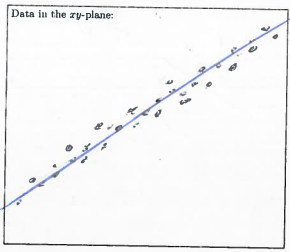
\includegraphics[width=0.6\textwidth]{./Figures/f201.png}
	\end{center}
	Here, $n$ individuals or events were observed, and two pieces of information were recorded for each individual/event (e.g., $n$ patients, $x_k$ stands for the score on a certain medical test, and $y_k$ stands for the score on a different test). Note that the data points are concentrated around a line. The data scientist has computed the slope of the line -- we will learn how fit lines through data later -- and now wants to project the data points onto it. One of the main advantages of this step is that the projected data will then be one-dimensional. That is, each point can then be described by one real number, namely its position along the line. This reduction can make a significant difference for the overall computational complexity of big data projects.
	
	We now derive how to project points \emph{orthogonally} onto a line. Let $L\subseteq\mathbb{R}^2$ be a line and let $w\in\mathbb{R}^2$ be a point that is not an element of $L$. Denote the projection of $w$ onto $L$ by $\wtd{w}$. To project orthogonally means that the line segment connecting $w$ and $\wtd{w}$ is orthogonal to $L$. Let $v$ be a vector that spans $L$, i.e. $L$ is the set of all scalar multiples of $V$,
	\[ L = \{ \lambda v \: | \: \lambda \in \mathbb{R} \} \subseteq \mathbb{R}^2 \:. \]
	This looks as follows, and the goal is now to find a formula for $\wtd{w}$ in terms of $v$ and~$w$.
	%\figbox{Orth. proj. onto a line:}
	\begin{center}
		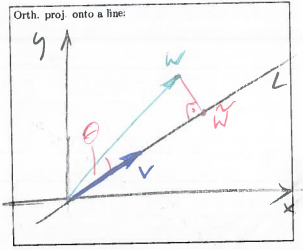
\includegraphics[width=0.6\textwidth]{./Figures/f202.png}
	\end{center}
	
	To visualise elements of $\mathbb{R}^2$, we are using two interpretations interchangeably: $w$ can be interpreted as a point, e.g.,
	\[ w = (1,2) \:, \]
	or as a vector,
	\[ w = \begin{bmatrix} 1 \\ 2 \end{bmatrix}, \]
	where the latter is often drawn as an arrow. Basing the arrow at the origin $(0,0)$ of the $xy$-plane, and interpreting it as ``move $1$ in the $x$ direction and $2$ in the $y$ direction'', we see that the vector $w$ points to the point $w$. This correspondence justifies switching freely between the two interpretations.
	
	Back to the task at hand, let us collect a few formulas for the right-angled triangle in the sketch:
	\begin{enumerate}
		\item \[ \cos \theta = \frac{ v \circ w }{||v||\,||w||} \]
		\hfill (cf. Remark~\ref{rem:vectors} (iv))
		\item \[ \cos \theta 
		= \frac{\text{length adjacent side}}{\text{length hypotenuse}} 
		= \frac{||\wtd{w}||}{||w||} \]
		\hfill (trig. identity for right-angled triangle)
		\item \[ \wtd{w} = \frac{||\wtd{w}||}{||v||} \, v \]
	\end{enumerate}
	Regarding the last formula: $\wtd{w}$ can be written as $\wtd{w}=\lambda v$ with $\lambda > 0$, since it lies on the side of $L$ in which $v$ points. To verify that the factor $\lambda = \rfrac{||\wtd{w}||}{||v||}$ is correct, we use the fact that $||\lambda v||=|\lambda| \,||v||$~:
	\[ \left|\left| \, \frac{||\wtd{w}||}{||v||} v  \, \right| \right|
	=  \left| \frac{||\wtd{w}||}{||v||} \right| ||v||
	=  \frac{||\wtd{w}||}{||v||} ||v||
	= ||\wtd{w}|| \qquad \text{\checkmark} \]
	Combining these formulas gives
	\begin{equation*}
	\wtd{w} \stackrel{(3)}{=} v \cdot \frac{||\wtd{w}||}{||v||}
	\stackrel{(2)}{=} v \cdot \frac{\cos\theta\,||w||}{||v||}
	\stackrel{(1)}{=} v \cdot \frac{\frac{ v \circ w }{||v||\,||w||}\,||w||}{||v||}
	= \frac{v \cdot (v \circ w)}{||v||^2} \:.
	\end{equation*}
	Both $v \circ w$ and $||v||^2 = v \circ v$ are scalars that can be written as matrix products via transposition of the first factor. Once all operations are regular products, associativity of matrix multiplication can be used. We find that the projection $w \mapsto \wtd{w}$ is carried out by multiplication with a $2 \times 2$ matrix:
	\[ \wtd{w} = \frac{v \cdot (v^\top \cdot w)}{v^\top \cdot v}
	= \frac{v \, v^\top}{v^\top \, v} \, w  = P_L \, w \:. \]
\end{application}

\begin{exercise}
\begin{enumerate}[(i)]
	\item Practise matrix multiplication by finding $AB$ and $BA$ for the matrices\footnote{For the difference $AB-BA$, you should obtain
	\[ \begin{bmatrix}
	10 & 7 & -20 \\ -23 & -9 & 39 \\ 1 & 3 & -1 
	\end{bmatrix}. \]} 
	\[ A = \begin{bmatrix}
	4 & 2 & -1 \\ -3 & -3 & 9 \\ 1 & 0 & 6
	\end{bmatrix}, \quad B = \begin{bmatrix}
	3 & 3 & -1 \\ 0 & -4 & 2 \\ 0 & 0 & 2
	\end{bmatrix}. \]
	\item Compute the matrix product 
	\[ \begin{bmatrix} 1 & 2 \end{bmatrix} 
	\begin{bmatrix} 3 & 4 \\ 5 & 6 \end{bmatrix}
	\begin{bmatrix} 7 \\ 8 \end{bmatrix}. \]
	The multiplication can be carried out in two different ways: $(AB)C$ and $A(BC)$ -- try both approaches and make sure that you obtain the same result.
	\item Consider the function $f(x)=x^2-2x-3$. This expression can also be written as $x^2 - 2 \cdot x^1 - 3 \cdot x^0$, since $x^0=1$. For matrices, the zeroth power is defined similarly: $A^0=I$, where $I$ is the identity matrix. Hence find $f(A)$ for the matrix\footnote{$f(A)=0$.}
	\[ A = \begin{bmatrix} -1 & 0 \\ 4 & 3	\end{bmatrix}. \]
	\item Find the angle between the two vectors\footnote{$\theta = \tfrac{\pi}{3}$.}
	\[ v = \begin{bmatrix} 2 & -1 & 0 & 1 \end{bmatrix}^\top,
	\quad w = \begin{bmatrix} 4 & 2 & 2 & 0 \end{bmatrix}^\top. \]
	\item Pick a $2 \times 3$ and a $3 \times 1$ matrix and check that property (iv) in~\ref{prop:matrix_mult} holds. Similarly, verify the statements made in~\ref{prop:det} for a few examples. (Be aware though that verifying examples does not constitute a proof!)
	\item Compute the determinants of\footnote{The determinants are $8,18,30$.}
	\[ \begin{bmatrix} 3 & 1 \\ -5 & 1 \end{bmatrix}, \quad
	\begin{bmatrix}	3 & 1 & -2 \\ -5 & 1 & 3 \\ 2 & 0 & 1 \end{bmatrix}, \quad
	\begin{bmatrix}
	3 & 1 & -2 & 3 \\ -5 & 1 & 3 & -4 \\ 2 & 0 & 1 & -1 \\ 1 & -5 & 3 & -3 
	\end{bmatrix} . \]
	\item Let $A$, $B$, $C$ be $n \times n$ matrices with the properties $AB=I$, $BC=I$, $CA=I$. Find $\tfrac13\left(A^2+B^2+C^2\right)$.
	\item Let $I$ be the $2 \times 2$ identity matrix. Show that for any $2 \times 2$ matrix\footnote{Consider a general matrix $A = \begin{bmatrix} a & b \\ c & d \end{bmatrix}$; multiply with $I$ in both orders; compare.} $A$, \[A \, I = I \, A = A\:.\] 
	\item The product $AB$ is not always the same as $BA$, but for some matrices we do have $AB=BA$ -- e.g., if one of the two is the zero matrix or the identity matrix. Perhaps there are more matrices that commute with a given matrix~$A$.
	
	Consider
	\[ A = \begin{bmatrix} 1 & 0 \\ -1 & 0	\end{bmatrix}. \]
	For which $2 \times 2$ matrices $X$ do we have\footnote{Matrices of the form
		\[ X = \begin{bmatrix} a & 0 \\ b & a+b \end{bmatrix}, \]
		where $a,b\in\mathbb{R}$, commute with $A$.} $AX=XA$ ?
	\item Show that\footnote{Prove by induction; use angle sum identities for trigonometric functions.}
	\[ \begin{bmatrix} \cos \theta & - \sin \theta \\ \sin \theta & \cos \theta \end{bmatrix}^n
	= \begin{bmatrix} \cos n\theta & - \sin n\theta \\ \sin n\theta & \cos n\theta \end{bmatrix}. \]
	\item Suppose you have to find the determinant of a $7 \times 7$ matrix that has no zero entries. You plan to reduce the problem to finding $3 \times 3$'s by applying Laplace's formula several times. How many $3 \times 3$ determinants do you have to compute?
	\item Find the two scalars $\lambda_1$ and $\lambda_2$ for which the determinant of 
	\[ A_{\lambda} = \begin{bmatrix}
	\lambda & 1 & 1 \\ 1 & \lambda & 1 \\ 1 & 1 & \lambda
	\end{bmatrix} \]
	is equal to zero\footnote{Computing this determinant with Sarrus' rule leads to a third-order algebraic expression in $\lambda$. To find its zeros, you first need to guess one solution -- property (ii) of~\ref{prop:det} should be helpful. The second value for $\lambda$ is $\lambda_2=-2$.}.
	\item Project the point $p=(\rfrac12,10)$ orthogonally onto the line\footnote{
	\[  \wtd{p} = \frac{1}{26}
	\begin{bmatrix} 1 & 5 \\ 5 & 25 \end{bmatrix} \begin{bmatrix} \rfrac12 \\ 10 \end{bmatrix}
	= \frac{50.5}{26}\begin{bmatrix} 1 \\ 5 \end{bmatrix}
	\approx \begin{bmatrix} 1.942 \\ 9.712 \end{bmatrix} \]}
	$L \: : \: y=5x$.
\end{enumerate}
\end{exercise}


\section{Systems of Linear Equations: Gaussian Elimination}
\label{sec:sys_lin_equ}
Suppose that the two equations
\begin{equation*}
\begin{cases}
\begin{array}{rcccccl}
2 & x & - & 3 & y & = & 7 \\
-2 & x & + & & y & = & 5
\end{array} \end{cases}
\end{equation*}
need to be satisfied simultaneously. Adding them together gives $-2y = 12$ and therefore $y = -6$. Now that $y$ is known, the first of the original equations reads $2x-3(-6) = 7$ and hence the solution is
\begin{equation}
\label{eq:sole_sol}
x = -\frac{11}{2}, \: y = -6 \:.
\end{equation}

\begin{remark}
\begin{enumerate}[(i)]
	\item The first equation above defines a line in the $xy$-plane, namely $y=\tfrac23x-\tfrac73$. Similarly, the second equation describes the line $y=2x+5$. With the computation above, we have found the intersection of those two lines.
	\item In order to convince yourself that it is permissible to add two equations together, think of two libra scales. Suppose that each of them is in balance. Then, taking the two objects from one scale and putting them onto the two arms of the other, the scale will still be in balance.
	\item The solution~\eqref{eq:sole_sol} above -- which consists of two equations -- can also be written as one vector equation:
	\[ \begin{bmatrix} x \\ y \end{bmatrix} 
	= \begin{bmatrix} -\tfrac{11}{2} \\ -6 \end{bmatrix}. \] 
\end{enumerate}
\end{remark}

\begin{definition}[Linear systems of equations] 
\label{def:lin_sys_equ}
A collection of equations of the form
\begin{equation*}
\begin{cases}
\begin{array}{ccccccccc}
a_{11} \: x_1 & + & a_{12} \: x_2 & + & a_{13} \: x_3 & \dots & + & a_{1n} \: x_n & = \: b_1 \\
a_{21} \: x_1 & + & a_{22} \: x_2 & + & a_{23} \: x_3 & \dots & + & a_{2n} \: x_n & = \: b_2 \\
\vdots & & & & \vdots & & & &\vdots \\
a_{m1} \: x_1 & + & a_{m2} \: x_2 & + & a_{m3} \: x_3 & \dots & + & a_{mn} \: x_n & = \: b_m 
\end{array} \end{cases}
\end{equation*}
is called a \emph{linear system of equations}. Here, $(x_1,x_2,\dots,x_n)$ are the variables, the $a_{ij}$ are the coefficients of the system, and $(b_1,b_2,\dots,b_m)$ is the right-hand side (RHS). If the RHS is zero, $b_1 = b_2 = \dots = b_m = 0$, then the system is called \emph{homogeneous}. A combination of variables $(x_1^*,x_2^*,\dots,x_n^*)$ that satisfies all $m$ equations simultaneously is called a \emph{solution} of the system.
\end{definition}

\begin{remark}
\begin{enumerate}[(i)]
\item For $n=2$ or $n=3$ the variables are often called $(x,y)$ or $(x,y,z)$.
\item Each equation demands that some ``linear combination'' of the variables -- that is, the variables multiplied by some coefficients and then added up -- be equal to some given value. If powers or square roots or other functions of the variables appear in an equation, then it is not linear and can not be solved with the theory developed in this chapter.
\item Such a system can have no solution, a unique solution, or many solutions.
\item We refer to the equations in the system as \emph{rows}, and the following definition lists modifications of a system that do not change the set of solutions. We have already used one such modification in the computation above: adding one row to another.
\end{enumerate}
\end{remark}

\begin{definition}[Elementary row operations]
	\label{def:ero}
The following \emph{row operations} on a system of equations do not change the set of its solutions.
\begin{enumerate}[(i)]
\item Add one row to another.
\item Multiply a row by a scalar different from zero.
\item Add the multiple of a row to another row.
\item Swap rows.
\end{enumerate}
\end{definition}

\begin{example}
\label{expl:lin_sys_equ}
Solve the system
\begin{equation*}
\begin{cases}
\begin{array}{rrrrrrr}
 x & - & y &  &  & = & 3 \phantom{\:.} \\
-3 x & + & 4 y & + & z & = & -1 \phantom{\:.} \\
2 x &  & & + & 7 z & = & -3 \:.
\end{array} \end{cases}
\end{equation*}
{\it Sol.:} We ``eliminate'' the terms $-3x$ and $2x$ by adding $3$ times the first row to the second and by subtracting $2$ times the first row from the third. This transformation is denoted ``$R2 \rightarrow R2 + 3 \cdot R1$'' and ``$R3 \rightarrow R3 - 2 \cdot R1$'', i.e. the arrow is to be read as ``is replaced with'':
\begin{equation}
\label{eq:first_3x3_example}
\begin{split}
\begin{array}{cc}
& ~~~\rightarrow~~~ \\
R2 \rightarrow R2 + 3 \cdot R1 & \\
R3 \rightarrow R3 - 2 \cdot R1 &
\end{array}
& \begin{cases}
\begin{array}{rrrrrrr}
x & - & y &  &  & = & 3 \\
 & & y & + & z & = & 8 \\
 & & 2 y & + & 7 z & = & -9 
\end{array} \end{cases} \\ 
\begin{array}{cc}
& ~~~\rightarrow~~~ \\
& \\
R3 \rightarrow R3 - 2 \cdot R2 &
\end{array}
& \begin{cases}
\begin{array}{rrrrrrr}
x & - & y &  &  & = & 3 \phantom{\:.} \\
& & y & + & z & = & 8 \phantom{\:.} \\
& & & & 5 z & = & -25 \:.
\end{array} \end{cases}  
\end{split}
\end{equation}
The last line yields $z = -5$, and one can then find $y$ and $x$ by back-substituting into the first two equations,
\[ x = 16, \: y = 13, \: z = -5 \:. \]
\end{example}

\begin{remark}
\begin{enumerate}[(i)]
\item The system in Definition~\ref{def:lin_sys_equ} can also be written in matrix form. Keeping in mind that an equation of two $n$-vectors amounts to $n$ equations, convince yourself that the following is equivalent to the system in~\ref{def:lin_sys_equ}.
\[
\begin{bmatrix}
a_{11} & a_{12} & a_{13} & \cdots & a_{1n} \\
a_{21} & a_{22} & a_{23} & \cdots & a_{2n} \\
\vdots & \vdots & \vdots & \ddots & \vdots \\
a_{m1} & a_{m2} & a_{m3 }& \cdots & a_{mn}
\end{bmatrix} \begin{bmatrix}
x_1 \\ x_2 \\ x_3 \\ \vdots \\ x_n
\end{bmatrix} = \begin{bmatrix}
b_1 \\ b_2 \\ \vdots \\ b_m
\end{bmatrix}.
\]
\item The transformation~\eqref{eq:first_3x3_example} via elementary row operations in the previous example is called \emph{Gaussian elimination}. We now define two standard matrix forms that are the goal of this process.
\end{enumerate}
\end{remark}

\begin{definition}[Augmented matrix, row echelon form, rank]
\end{definition}
\begin{enumerate}[(i)]
	\item The \emph{augmented matrix} for the system in Definition~\ref{def:lin_sys_equ} is
	\[ [A\:|\:b] = \left[\begin{array}{ccccc|c}
	a_{11} & a_{12} & a_{13} & \dots & a_{1n} & b_1 \\
	a_{21} & a_{22} & a_{23} & \dots & a_{2n} & b_2 \\
	\vdots & \vdots & \vdots &\ddots & \vdots & \vdots \\
	a_{m1} & a_{m2} & a_{m3} & \dots & a_{mn} & b_m 
	\end{array}\right], \]
	and it can be subjected to elementary row operations the same way as fully written-out systems of linear equations.
	\item The first nonzero entry in a row of a matrix is called the \emph{leading entry}. A matrix (augmented or not) of the form
	\[ \left[\begin{array}{ccccccc}
	\rowcolor{blue!50}
	(*) & \phantom{(*)} & \phantom{(*)} & \phantom{(*)} & \phantom{(*)} & \phantom{(*)} & \phantom{(*)} \\
	\cellcolor{red!30} & \cellcolor{red!30} & \cellcolor{blue!50}(*) & \cellcolor{blue!50} & \cellcolor{blue!50} & \cellcolor{blue!50} & \cellcolor{blue!50} \\
	\cellcolor{red!30} & \cellcolor{red!30} & \cellcolor{red!30} & \cellcolor{blue!50}(*) & \cellcolor{blue!50}& \cellcolor{blue!50} & \cellcolor{blue!50} \\ 
	\cellcolor{red!30} & \cellcolor{red!30}0 & \cellcolor{red!30} & \cellcolor{red!30} & \cellcolor{red!30} & \cellcolor{red!30} & \cellcolor{blue!50}(*) \\ 
	\rowcolor{red!30}
	& & & & & & 
	\end{array}\right], \]
	where all entries in the red (light) part are zero and the $(*)$ stand for leading entries, is said to be in \emph{row echelon form} (REF). That is, zero rows are at the bottom and for the remaining rows -- say there are $r$ of them -- we have
	\[ j_1 < j_2 < j_3 < \dots < j_r \:, \]
	where $j_i$ is the column index of the leading entry in row $i$ (e.g., in the schematic example above, $j_1=1,j_2=3,j_3=4,j_4=7$).
	\item A matrix in REF is further said to be in \emph{reduced row echelon form} (RREF), if all leading entries are $1$ and if each leading entry is the only nonzero entry in its column.
	\item The \emph{rank} of a matrix is the number of nonzero rows in its REF.
\end{enumerate}

\begin{example}
\label{expl:augm_matrix}
\begin{enumerate}[(i)]
	\item The matrices
	\[ \begin{bmatrix}
	-3 & 0 & 1 \\ 0 & 0 & 2 \\ 0 & 0 & 0
	\end{bmatrix}, \begin{bmatrix}
	0 & 1 & 1 & 0 \\ 0 & 0 & 2 & -3 
	\end{bmatrix}, \begin{bmatrix}
	1 & 2 & 3 \\ 0 & 4 & 5 \\ 0 & 0 & 6 \\ 0 & 0 & 0
	\end{bmatrix} \]
	all are in REF and have ranks 2, 2, and 3. If those matrices are the outcome of Gaussian elimination, then the original matrices have the same rank -- the rank does not change under elementary row operations, but it can be read off directly only from the REF. The matrices
	\[ \begin{bmatrix}
	-3 & 0 & 1 \\ 0 & 0 & 0 \\ 0 & 0 & 2
	\end{bmatrix}, \begin{bmatrix}
	1 & 2 & 3 \\ 0 & 4 & 5 \\ 0 & 6 & 7 \\ 0 & 0 & 8
	\end{bmatrix} \]
	are not in REF.
	\item The matrices
	\[ I, \begin{bmatrix}
	1 & -2 & 0 \\ 0 & 0 & 1 \\ 0 & 0 & 0
	\end{bmatrix}, \begin{bmatrix}
	0 & 1 & 0 & 2 \\ 0 & 0 & 1 & -3 
	\end{bmatrix} \]
	all are in RREF, but the matrices in (i) are not.
	\item In Example~\ref{expl:lin_sys_equ}, we have transformed
	\[ \left[\begin{array}{ccc|c}
		1 & -1 & 0 & 3 \\
		-3 & 4 & 1 & -1 \\
		2 & 0 & 7 & -3 
	\end{array}\right] \qquad \stackrel{\eqref{eq:first_3x3_example}}{\rightarrow} \qquad \left[\begin{array}{ccc|c}
	1 & -1 & 0 & 3 \\
	0 & 1 & 1 & 8 \\
	0 & 0 & 5 & -25 
	\end{array}\right]. \]
	The transformed augmented matrix is in REF and has rank $3$. Therefore, the original augmented matrix has rank $3$ as well. Including the vector of variables that is dropped when writing systems as augmented matrices, the last line reads
	\[ \begin{bmatrix}
	0 & 0 & 5
	\end{bmatrix} \begin{bmatrix}
	x \\ y \\ z
	\end{bmatrix} = -25 \:, \]
	i.e.,  $0 \cdot x + 0 \cdot y + 5 \cdot z = 5z = -25$. With back-substitution, one can then find $x$ and $y$ as before. Another option is to bring the augmented matrix into reduced row echelon form:
	\[ 
	\begin{array}{ccc}
	\left[\begin{array}{ccc|c}
	1 & -1 & 0 & 3 \\
	0 & 1 & 1 & 8 \\
	0 & 0 & 5 & -25 
	\end{array}\right] & \stackrel{R3 \rightarrow \rfrac15 \cdot R3}{\rightarrow} \qquad & \left[\begin{array}{ccc|c}
	1 & -1 & 0 & 3 \\
	0 & 1 & 1 & 8 \\
	0 & 0 & 1 & -5 
	\end{array}\right] \\ & & \\
	& \stackrel{R2 \rightarrow R2 - R3}{\rightarrow} \qquad & \left[\begin{array}{ccc|c}
	1 & -1 & 0 & 3 \\
	0 & 1 & 0 & 13 \\
	0 & 0 & 1 & -5 
	\end{array}\right] \\ & & \\
	& \stackrel{R1 \rightarrow R1 + R2}{\rightarrow} \qquad & \left[\begin{array}{ccc|c}
	1 & 0 & 0 & 16 \\
	0 & 1 & 0 & 13 \\
	0 & 0 & 1 & -5 
	\end{array}\right].
	\end{array}	\]
	The augmented matrix now corresponds to
	\[ \begin{bmatrix}
	16 \\ 13 \\ -5
	\end{bmatrix} = \begin{bmatrix}
	1 & 0 & 0 \\ 0 & 1 & 0 \\ 0 & 0 & 1 
	\end{bmatrix} \begin{bmatrix}
	x \\ y \\ z
	\end{bmatrix} = \begin{bmatrix}
	x \\ y \\ z
	\end{bmatrix}, \]
	from which -- for this example -- the solution can be read off directly.
	\item To solve the system
	\begin{equation*}
	\begin{cases}
	\begin{array}{rrrrrrr}
	-3x &   &    & + & 3z & = & 4 \phantom{\:,} \\
	 3x & + & 5y & + &  z & = & 0 \phantom{\:,} \\
	 -x & + & 5y & + & 5z & = & 3 \:,
	\end{array} \end{cases} 
	\end{equation*}
	we construct the augmented matrix and transform it with elementary row operations. It is preferable to have an entry $1$ in the upper left corner -- therefore, we start by swapping row 3 to the top and multiply it by $-1$~:
	\[ 
	\begin{array}{ccc}
	\left[\begin{array}{ccc|c}
	-3 & 0 & 3 & 4 \\
	3  & 5 & 1 & 0 \\
	-1 & 5 & 5 & 3 
	\end{array}\right] & \stackrel{R3 \leftrightarrow R1}{\rightarrow} \qquad & \left[\begin{array}{ccc|c}
	-1 & 5 & 5 & 3 \\
	3 & 5 & 1 & 0 \\
	-3 & 0 & 3 & 4 
	\end{array}\right] \\ & & \\
	& \stackrel{R1 \rightarrow - R1}{\rightarrow} \qquad & \left[\begin{array}{ccc|c}
	1 & -5 & -5 & -3 \\
	3 & 5 & 1 & 0 \\
	-3 & 0 & 3 & 4 
	\end{array}\right] \\ & & \\
	& \stackrel{R2 \rightarrow R2 -3 R1}{\rightarrow} \qquad & \left[\begin{array}{ccc|c}
	1 & -5 & -5 & -3 \\
	0 & 20 & 16 & 9 \\
	-3 & 0 & 3 & 4 
	\end{array}\right] \\ & & \\
	& \stackrel{R3 \rightarrow R3 + 3 R1}{\rightarrow} \qquad & \left[\begin{array}{ccc|c}
	1 & -5 & -5 & -3 \\
	0 & 20 & 16 & 9 \\
	0 & -15 & -12 & -5 
	\end{array}\right] \\ & & \\
	& \stackrel{R3 \rightarrow R3 + \rfrac{3}{4} R2}{\rightarrow} \qquad & \left[\begin{array}{ccc|c}
	1 & -5 & -5 & -3 \\
	0 & 20 & 16 & 9 \\
	0 & 0 & 0 & \rfrac{7}{4} 
	\end{array}\right].
	\end{array}	\]
	The last line reads
	\[ \rfrac74 = \begin{bmatrix}
	0 & 0 & 0
	\end{bmatrix} \begin{bmatrix}
	x \\ y \\ z
	\end{bmatrix} = 0 \cdot x + 0 \cdot y + 0 \cdot z = 0 \:, \]
	 which is never true -- for no combination $(x,y,z)$. Hence the system of linear equations does not have a solution.
\end{enumerate}
\end{example}

\begin{remark}
As the previous example has shown, if the REF of the augmented matrix has a row of zeros on the left-hand side, but the corresponding entry on the right is different from zero, then the system does not have a solution. A formal way of expressing this is
\[ \rank A < \rank[A\:|\:b] \]
-- the rank of the coefficient matrix alone is smaller than the rank of the augmented matrix.
\end{remark}

\begin{theorem}[Solutions of systems of linear equations]
\label{thm:rank_sols}
Suppose a system of $m$ linear equations in $n$ variables is given. That is, the coefficient matrix $A$ of the system is of size $m \times n$. Denote the right-hand side of the system by $b$. Then:
\begin{enumerate}[(i)]
\item If	
\[ \rank A < \rank [A\:|\:b] \:, \]	
then the system does not have a solution.
\item If	
\[ \rank A = \rank [A\:|\:b]  = n \:, \]	
then the system has a unique solution.
\item If	
\[ \rank A = \rank [A\:|\:b] < n \:, \]	
then the system has many solutions.
\item Those cases cover all possibilities, as $\rank A$ can not be greater than $n$ or $\rank [A\:|\:b]$.
\end{enumerate}
\end{theorem}

\begin{example}
\label{expl:systems_of_eqns}
\begin{enumerate}[(i)]
	\item Example (iii) of~\ref{expl:augm_matrix} corresponds to the unique-solution case of Theorem~\ref{thm:rank_sols}, and example (iv) to the no-solution case. The third case is demonstrated in the following examples.
	\item Let us re-do Example~\ref{expl:augm_matrix} (iv) with the right-hand side 
	$b = \begin{bmatrix} -9 & 8 & -4 \end{bmatrix}^\top.$
	The same row operations as before lead to
\[	\left[\begin{array}{ccc|c}
			-3 & 0 & 3 & -9 \\
			3  & 5 & 1 & 8 \\
			-1 & 5 & 5 & -4 
	\end{array}\right] \quad \stackrel{\dots}{\rightarrow} \quad \left[ \begin{array}{ccc|c}
			1 & -5 & -5 & 4 \\
			0 & 20 & 16 &  -4 \\
			0 & -15 & -12 & 3 
		\end{array}\right]. \]
	The third row is a multiple of the second, and the next operation, $R3 \rightarrow R3 + \rfrac{3}{4} R2$, eliminates the third row altogether. We then continue to bring the system into RREF:
	\[\begin{array}{ccc}
		\left[\begin{array}{ccc|c}
			1 & -5 & -5 & 4 \\
			0  & 20 & 16 & -4 \\
			0 & 0 & 0 & 0 
		\end{array}\right] & \stackrel{R2 \rightarrow \rfrac{1}{20}R2}{\rightarrow} \qquad & \left[\begin{array}{ccc|c}
			1 & -5 & -5 & 4 \\
			0 & 1 & \rfrac45 & -\rfrac15 \\
			0 & 0 & 0 & 0 
		\end{array}\right] \\ & & \\
		& \stackrel{R1 \rightarrow R1 + 5 R2}{\rightarrow} \qquad & \left[\begin{array}{ccc|c}
			1 & 0 & -1 & 3 \\
			0 & 1 & \rfrac45 & -\rfrac15 \\
			0 & 0 & 0 & 0 
		\end{array}\right]. 
	\end{array}	\]
	The solution $\begin{bmatrix} x & y & z \end{bmatrix}^\top$ is now obtained as follows. Variables corresponding to columns that do not have a leading entry can be chosen freely. This is expressed using a parameter,
	\[ z = t \qquad (t \in \mathbb{R}) \:. \]
	To obtain an expression for $y$, we use the row whose leading entry is in the column corresponding to $y$:
	\[ y + \tfrac45 z = -\tfrac15 \quad \rightarrow \quad y = -\tfrac15-\tfrac45t \:. \]
	Similarly for $x$:
	\[ x - z = 3 \quad \rightarrow \quad x = 3 + t \:. \]
	Therefore, the answer is
	\[  \left\{ \begin{array}{l}
	x = 3 + t \\
	y = -\tfrac15 -\tfrac45t \\
	z = t \:,
	\end{array} \right. \qquad (t\in\mathbb{R}), \]
	which can also be written as
	\[ \begin{bmatrix}
	x \\ y \\z
	\end{bmatrix} = \begin{bmatrix}
	3 \\ -\rfrac15 \\ 0 
	\end{bmatrix} + t \cdot \begin{bmatrix}
	1 \\ - \rfrac45 \\ 1
	\end{bmatrix}, \qquad (t\in\mathbb{R}). \]
	The latter form is the equation of a line -- namely the line of common points of the three planes $-3x +3z=-9$, $3x+5y+z=8$, $-x+5y+5z=-4$.
	\item For the system
	\begin{equation*}
	\begin{cases}
	\begin{array}{rrrrrrr}
	-6x_1 & +6x_2 & +2x_3 & -2x_4 & = & 2 \phantom{\:,}\\
	-9x_1 & +8x_2 & +3x_3 & -2x_4 & = & 3 \phantom{\:,}\\
	-3x_1 & +2x_2 & +\phantom{1}x_3 &  & = & 1 \phantom{\:,}\\
	-15x_1 & +14x_2 & +5x_3 & -4x_4 & = & 5 \:,
	\end{array} \end{cases}
	\end{equation*}
	Gaussian elimination leads to the REF 
	\[ \left[ \begin{array}{cccc|c}
		-3 & 2 & 1 &  0 & 1 \\
		 0 & 2 & 0 & -2 & 0 
	\end{array} \right] \]
	(dropping two rows of zeros) and to the RREF
	\[ \left[ \begin{array}{cccc|c}
		1 & 0 & -\rfrac13 & -\rfrac23 & -\rfrac13 \\
		0 & 1 & 0 & -1 & 0 
	\end{array} \right]. \]
	The solution is
	\[ \left\{ \begin{array}{l}
	x_1 = \tfrac13 (t+2s-1) \\
	x_2 = s \\
	x_3 = t \\
	x_4 = s \:,
	\end{array} \right. \]
	where $t,s\in\mathbb{R}.$
\end{enumerate}
\end{example}

\begin{exercise}
\begin{enumerate}[(i)]
	\item Fill in the Gaussian elimination steps for Example~\ref{expl:systems_of_eqns} (iii) (careful: the RREF of a matrix is unique, but the REF is not -- therefore, the REF you find may differ from the one given above).
	\item Find $\rank A$ and $\rank [A\:|\:b]$ for the augmented matrices
	\[ \left[ \begin{array}{cc|c}
	1 & 0 & \rfrac13 \\
	1 & 1 & \rfrac13 
	\end{array} \right], \quad
	\left[ \begin{array}{ccc|c}
	1 & 2 & 3 & 4 \\
	0 & 5 & 6 & 7 \\
	0 & 0 & 8 & 9 \\
	2 & 5 & 7 & 3 
	\end{array} \right], \quad
	\left[ \begin{array}{cccc|c}
	3 & 2 & 0 & 5 & 0 \\
	3 & -2 & 3 & 6 & -1 \\
	2 & 0 & 1 & 5 & -3 \\
	1 & 6 & -4 & -1 & 4 
	\end{array} \right], \]
	and state for each case whether we have no solution, a unique solution, or infinitely many solutions\footnote{
\begin{center}
	\begin{tabular}{ l | c | c | c | c}
		 & ~$n$~ & $\rank A$ & $\rank [A\:|\:b]$ &  \# sol. \\ \hline
		(i) & 2 & 2 & 2 & 1 \\ \hline
		(ii) & 3 & 3 & 4 & 0 \\ \hline
		(iii) & 4 & 3 & 3 & $\infty$ \\
		\hline
	\end{tabular}
\end{center}}.
	\item Find all solutions of the homogeneous system\footnote{Using the parameter $t\in\mathbb{R}$, we obtain $(x,y,z)=(-2t,-2t,t)$.}
	\[ \begin{cases}	
		\begin{array}{rrrrrrr}
			4x & -2y & +4z & = & 0 \phantom{\:.}\\
			   &  +y & +2z & = & 0 \phantom{\:.}\\
			3x &  -y & +4z & = & 0 \:. 
		\end{array} \end{cases} \]
	\item Convince yourself of the fact that homogeneous systems always have a solution, i.e. at least one solution\footnote{The vector 
	\[ \begin{bmatrix} x & y & z \end{bmatrix}^\top
	=  \begin{bmatrix} 0 & 0 & 0 \end{bmatrix}^\top, \]
	satisfies all three equations. One can also argue more abstractly that the no-solution case in Theorem~\ref{thm:rank_sols} never happens if $b=0$.}.
	\item Find all solutions of the inhomogeneous system
	\[ \begin{cases}	
	\begin{array}{rrrrrrr}
	4x & -2y & +4z & = & -3 \phantom{\:.}\\
	-x &  +y & +2z & = & 1 \phantom{\:.}\\
	3x &  -y & +4z & = & 7 \:.
	\end{array} \end{cases} \]
	\item An equation $a_1 x + a_2 y + a_3 z = b$ describes a plane in $\mathbb{R}^3$ (just as $a_1x+a_2y=b$ describes a line in $\mathbb{R}^2$; here, $b\in\mathbb{R}$). For example, $y = 0$ describes the $xz$-plane. Think about this interpretation for a moment and connect it to solving systems of equations, i.e., finding simultaneous solutions of several equations. For example, try to picture different arrangements of three planes such that they have no point in common, exactly one point in common, and infinitely many points in common.
	\item Find $\alpha$ such that
	\[ \begin{cases}
	\begin{array}{rrrrrrr}
	5x & -3y & = & 2 \\
	-x & +2y & = & 1 \\
	-4x & +4y & = & \alpha 
	\end{array} \end{cases} \]
	has a solution\footnote{Bring the system in REF using Gaussian elimination as usual. Then choose $\alpha$ such that we are not in the no-solution case of Theorem~\ref{thm:rank_sols}.}.
	\item Find $\alpha, \beta$ such that
	\[ \begin{bmatrix}
	\alpha & 1 & 1 \\ 1 & \beta & 1 \\ 1 & 3\beta & 1
	\end{bmatrix} \begin{bmatrix} x_1 \\ x_2 \\ x_3
	\end{bmatrix} = \begin{bmatrix} 4 \\ 3 \\ 4	\end{bmatrix} \]
	has no solution, a unique solution, infinitely many solutions\footnote{Unique solution if $\alpha\not=1$ and $\beta\not=0$. Infinitely many solutions if $\alpha=1$ and $\beta=\rfrac13$. Otherwise, no solutions.}.
	\item In the last exercise of the previous section, you were asked to orthogonally project the point $p=(\rfrac12,10)$ onto the line $L \: : \: y=5x$. Now consider the following two different types of projections.
	\begin{enumerate}[(a)]
		\item $P_{L,x} \: : \: p=(\rfrac12,10) \mapsto \wtd{p}=(2,10)$ 
				\hfill \text(projection in the $x$ direction)
		\item $P_{L,y} \: : \: p=(\rfrac12,10) \mapsto \wtd{p}=(\rfrac12,\rfrac52)$
				\hfill \text(projection in the $y$ direction)
\end{enumerate}
	Sketch the action of the three different types of projections and find the matrices $P_{L,x},P_{L,y}$. What is the advantage of orthogonal projection over projection along the coordinate axes\footnote{\[
		\begin{bmatrix} a & b \\ c & d \end{bmatrix} \begin{bmatrix} x \\ y \end{bmatrix} 
		= \begin{bmatrix} ax+by \\ cx+dy \end{bmatrix} \stackrel{\text{!}}{=}
		P_{L,x} \begin{bmatrix} x \\ y \end{bmatrix}
		= \begin{bmatrix} \frac15y \\ y \end{bmatrix} 
		\quad \Rightarrow \quad 
		P_{L,x} = \begin{bmatrix} 0 & \rfrac15 \\ 0 & 1 \end{bmatrix} \]
	Alternatively, one can think about where the standard vectors 
	$\begin{bmatrix} 1 & 0 \end{bmatrix}^\top$ and
	$\begin{bmatrix} 0 & 1 \end{bmatrix}^\top$ get mapped to: 
	\[ P_{L,y} \: : \: \begin{bmatrix} 1 \\ 0 \end{bmatrix}
	\mapsto \begin{bmatrix} 1 \\ 5 \end{bmatrix}, \quad 
	\begin{bmatrix} 0 \\ 1 \end{bmatrix}
	\mapsto \begin{bmatrix} 0 \\ 0 \end{bmatrix} 
	\quad \Rightarrow \quad 
	P_{L,y} = \begin{bmatrix} 1 & 0 \\ 5 & 0 \end{bmatrix}. \]}?
\end{enumerate}
\end{exercise}


\section{Eigenvalues and Eigenvectors}

\begin{definition}[Eigenvalues and eigenvectors]
	Let $A$ be a $n \times n$ square matrix. A scalar $\lambda \in \mathbb{R}$ is called an \emph{eigenvalue} of $A$, if there exists a $n$-vector $v\not=0$ with 
	\[ Av = \lambda v \:. \]
	Such a vector $v$ is called an \emph{eigenvector} of $A$.
\end{definition}

\begin{remark}
\label{rem:ev}
\begin{enumerate}[(i)]
	\item In this section, all matrices are square, of size $n \times n$, and vectors are of the corresponding size $n$. 
	\item The vector on the left-hand side of the eigenvalue equation above is obtained via matrix multiplication. The vector on the right is found by scalar multiplication, which is much easier to compute. This observation already suggests that eigenvalues and eigenvectors are useful for simplifying matrix computations.
	\item The condition $v\not=0$ for eigenvectors is crucial. Indeed, for the zero vector, we have
	\[ A0 = 0 =\lambda 0 \]
	for any square matrix $A$ and for any scalar $\lambda$. Therefore, eigenvectors are nonzero by definition (otherwise, any $\lambda\in\mathbb{R}$ would be an eigenvalue). However, eigen\emph{values} can be zero: If there exists $v\not=0$ such that
	\[ Av= 0 = 0 \cdot v \:, \]
	then $v$ is an eigenvector of $A$ with eigenvalue $\lambda=0$ (where the first $0$ in the equation stands for zero vector and the second $0$ for the number zero).
	\item If $v$ is an eigenvector of $A$, then any nonzero multiple of $v$ is an eigenvector with the same eigenvalue: If we scalar-multiply $v$ by $\mu\not=0$, then
	\[ A(\mu v) = \mu (Av) = \mu (\lambda v) = \lambda (\mu v) \:. \]
	\item An approach to computing eigenvalues will be given by Theorem~\ref{thm:eigenvalues} below. That theorem and the results in the preceding lemma provide good opportunities to present a few proofs.
\end{enumerate}
\end{remark}

\begin{lemma}
\label{lem:rank_det}
For a $n \times n$ matrix $M$, we have:
\begin{enumerate}[(i)]
	\item There exists $v\not=0$ with $Mv=0 \quad \Longleftrightarrow \quad \rank M<n$~.
	\item The determinant of $M$ does not change when $M$ is subjected to elementary row operation (iii) in Definition~\ref{def:ero} -- adding the multiple of a row to another row.
	\item Each time two rows are swapped, the determinant changes by a factor of $-1$.
	\item $\quad \rank M <n \quad \Longleftrightarrow \quad \det M =0$~.
\end{enumerate}
\end{lemma}
\begin{proof}
\begin{enumerate}[(i)]
	\item Note that $\rank M = \rank [M\:|\:0]$, and we are therefore either in case (ii) or in case (iii) of Theorem~\ref{thm:rank_sols}. Note further that the zero vector $w=0$ solves $Mw=0$. If $\rank M = n$, this solution is unique by~\ref{thm:rank_sols} -- that is, there are no other solutions and hence no nonzero solutions. If $\rank M < n$, there are other solutions -- that is, nonzero solutions do exist in that case.
	\item Denote the rows of $M$ by $r^{(1)},r^{(2)},\dots,r^{(n)}$, and let $B$ be the matrix obtained by adding $\mu$ times the $q$-th row to the $p$-th row, where $p \not= q$:
	\[ M = \begin{bmatrix}
	--r^{(1)}-- \\
	--r^{(2)}-- \\
	\vdots \\
	--r^{(n)}--
	\end{bmatrix}, \qquad B = \begin{bmatrix}
	--r^{(1)}-- \\
	\vdots \\
	--r^{(p-1)}-- \\
	-\,r^{(p)} + \mu r^{(q)}\,- \\
	--r^{(p+1)}-- \\
	\vdots \\
	--r^{(n)}--
	\end{bmatrix}. \]
	To show that $\det B = \det M$, we apply Laplace's formula developing along the $p$-th row of $B$. As in the previous section, the matrix $\wtd{A}_{ij}$ is the $(n-1) \times (n-1)$ matrix obtained by deleting the $i$-th row and the $j$-th column from $A$:
	\begin{equation*}
	\begin{split}
	\det B & = \sum_{j=1}^n (-1)^{p+j} \left( r_j^{(p)} + \mu r_j^{(q)} \right) \det \wtd{B}_{pj} \\
	& = \sum_{j=1}^n (-1)^{p+j} \left( r_j^{(p)} + \mu r_j^{(q)} \right) \det \wtd{M}_{pj} \\
	& = \sum_{j=1}^n (-1)^{p+j} r_j^{(p)} \det \wtd{M}_{pj} + \sum_{j=1}^n (-1)^{p+j} \mu r_j^{(q)} \det \wtd{M}_{pj} \\
	& = \det M + \det \left( \begin{bmatrix}
	r^{(1)} \\ \vdots \\ r^{(q)} \\ \vdots \\ \mu r^{(q)} \\ \vdots \\ r^{(n)}
	\end{bmatrix}\right) = \det M + 0 = \det M \:,
	\end{split}
	\end{equation*}
	where the simplification in the last line is due to property (ii) of~\ref{prop:det}. We have shown that the determinant does not change when a multiple of a row is added to another row.
	\item By induction over $n$~:
	\begin{itemize}
		\item[$\mathbf{n=2}$~:]
		\[ \begin{vmatrix}
		c & d \\ a & b
		\end{vmatrix} = bc-ad = - \begin{vmatrix}
		a & b \\ c & d
		\end{vmatrix} \qquad \text{\checkmark} \]
		\item[$\mathbf{n=3}$~:] Suppose two rows of a $3 \times 3$ matrix have been swapped. Apply Laplace's formula in the row that has not changed. In each of the three $2 \times 2$ matrices, the rows have been swapped, and we therefore -- cf. the $n=2$ case above -- obtain an overall factor of $-1$.
		\item[$\mathbf{n=4}$~:] Suppose two rows of a $4 \times 4$ matrix have been swapped. Apply Laplace's formula in one of the rows that has not changed. In each of the four $3 \times 3$ matrices, two rows have been swapped, and we therefore -- cf. the $n=3$ case above -- obtain an overall factor of $-1$.
  		\item[$\mathbf{n>4}$~:] Via repetition of the step $n \rightsquigarrow n + 1$, the statement follows for all $n\geq2$.
	\end{itemize}
	\item First suppose that $M$ is in REF. Square matrices in REF have only zero entries below the diagonal. Therefore, $M$ is a upper diagonal matrix and its determinant is the product of its diagonal entries. If $\rank M < n$, then at least one diagonal entry is equal to zero, and thus $\det M = 0$. If $\rank M = n$, then none of the diagonal entries is zero, and therefore $\det M \not= 0$. Hence statement (iv) is true for REF matrices. Since all matrices can be brought into REF by swapping rows and adding multiples of rows to other rows, the general case follows from (ii) and (iii).
\end{enumerate}
\end{proof}

\begin{theorem}[Eigenvalue equation]
\label{thm:eigenvalues}	
	If $\lambda$ is an eigenvalue of $A$, then
	\[ \det(A - \lambda I) = 0 \:. \]
	The converse is also true: If $\det(A - \lambda I) = 0$, then $\lambda$ is an eigenvalue of $A$. The above equation -- a condition on the parameter $\lambda$ -- is called the \emph{eigenvalue equation} of $A$.
\end{theorem}
\begin{proof}
	\[ \begin{array}{cccrlcc}
	\lambda \text{~eigenvalue of~}A &\stackrel{\text{def.}}{\Longleftrightarrow} & & Av & = \lambda v & & (\text{for some~}v\not=0) \\	
	&\Longleftrightarrow & & Av - \lambda v & = 0 & & (\text{for some~}v\not=0) \\	
	&\Longleftrightarrow & & (A - \lambda I)v & = 0 & & (\text{for some~}v\not=0) \\
	&\stackrel{\text{Lemma~\ref{lem:rank_det} (i)}}{\Longleftrightarrow} & & \rank (A - \lambda I) & < n & & \\	
	&\stackrel{\text{\ref{lem:rank_det} (iv)}}{\Longleftrightarrow} & & \det(A - \lambda I) & = 0 & & 
	\end{array} \]
\end{proof}

\begin{example}
\label{expl:evs}
	\begin{enumerate}[(i)]
	\item Find the eigenvalues and eigenvectors of
		\[ A = \begin{bmatrix}
		1 & 5 \\ 10 & -4 
		\end{bmatrix}. \]
		{\it Sol.:}
		The eigenvalue equation is 
		\begin{equation*}
		\begin{split}
		0 & = \det (A-\lambda I) =\det \left( 
		\begin{bmatrix}
		1 & 5 \\ 10 & -4
		\end{bmatrix} - \lambda \begin{bmatrix}
		1 & 0 \\ 0 & 1
		\end{bmatrix}
		\right) \\ 
		& = \begin{vmatrix}  
		1 - \lambda & 5 \\ 10 & -4 - \lambda
		\end{vmatrix} = (1-\lambda)(-4-\lambda)-10 \cdot 5\\ 
		& = \lambda^2 +3\lambda -54 = (\lambda+9)(\lambda-6) \:,
		\end{split}
		\end{equation*}
		and its roots 
		\[ \begin{cases} \lambda_1 = -9 \\ \lambda_2 = 6 \:. \end{cases}  \]
		are the eigenvalues of $A$.
		
		The eigenvector $v_1$ is found  by solving $Av_1=\lambda_1v_1 \leftrightarrow (A-\lambda_1 I)v_1=0$~:
		\[\begin{array}{ccc}
		\left[\begin{array}{cc|c}
		1-\lambda_1 & 5 & 0 \\
		10 & -4-\lambda_1& 0 \\
		\end{array}\right] & = \qquad & \left[\begin{array}{cc|c}
		10 & 5 & 0 \\
		10 & 5 & 0 
		\end{array}\right] \\ & & \\
		& \stackrel{R2 \rightarrow R2 - R1}{\rightarrow} \qquad & 
		\left[\begin{array}{cc|c}
		10 & 5 & 0 \\
		0 &  0 & 0 
		\end{array}\right]
		.\end{array} \]
		The first row of that system corresponds to 
		\[ 10 x + 5 y = 0 \:, \]
		which gives $y = - 2 x$. As was pointed out in Remark~\ref{rem:ev}, multiples of eigenvectors are eigenvectors as well -- this explains why the above system does not determine $x$ and $y$ uniquely; for any solution $(x,y)$ and any constant factor $c\not=0$, the scalar multiple $(cx,cy)$ is a solution as well. Choosing $x=1$, we obtain
		\[v_1 = \begin{bmatrix}
		1 \\ -2
		\end{bmatrix} \qquad (\lambda_1 = -9) \:. \]
				
		For the second eigenvector, we solve $(A-\lambda_2 I)v_2=0$~:
		\[\begin{array}{ccc}
		\left[\begin{array}{cc|c}
		1-\lambda_2 & 5 & 0 \\
		10 & -4-\lambda_2& 0 \\
		\end{array}\right] & = \qquad & \left[\begin{array}{cc|c}
		-5 & 5 & 0 \\
		10 & -10 & 0 
		\end{array}\right] \\ & & \\
		& \stackrel{R2 \rightarrow R2 + 2 R1}{\rightarrow} \qquad & 
		\left[\begin{array}{cc|c}
		-5 & 5 & 0 \\
		0 &  0 & 0 
		\end{array}\right].
		\end{array}	\]
		Here, the first row reads
		\[ -5 x + 5 y = 0 \]
		and leads to
		\[v_2 = \begin{bmatrix}
		1 \\ 1
		\end{bmatrix} \qquad (\lambda_2 = 6) \:. \]
	\item Verify the results from the previous example.\\
		{\it Sol.:}
		\[ Av_1 = \begin{bmatrix}
		1 & 5 \\ 10 & -4 
		\end{bmatrix} \begin{bmatrix}
		1 \\ -2
		\end{bmatrix} = \begin{bmatrix}
		1-10 \\ 10 + 8
		\end{bmatrix} = \begin{bmatrix}
		-9 \\ 18
		\end{bmatrix} = -9 \begin{bmatrix}
		1 \\ -2
		\end{bmatrix} = \lambda_1 v_1
		\qquad \text{\checkmark} \]
		\[ Av_2 = \begin{bmatrix}
		1 & 5 \\ 10 & -4 
		\end{bmatrix} \begin{bmatrix}
		1 \\ 1
		\end{bmatrix} = \begin{bmatrix}
		1+5 \\ 10 - 4
		\end{bmatrix} = \begin{bmatrix}
		6 \\ 6
		\end{bmatrix} = 6 \begin{bmatrix}
		1 \\ 1
		\end{bmatrix} = \lambda_2 v_2
		\qquad \text{\checkmark} \]
	\item Find the eigenvalues and eigenvectors of
		\[ M = \begin{bmatrix}
		-5 & 0 & 7 \\ 6 & 2 & -6 \\ -4 & 0 & 6 
		\end{bmatrix}. \]
		{\it Sol.:}
		\begin{equation*}
		\begin{split}
		0 & = \det (M-\lambda I) = \begin{vmatrix}  
			-5-\lambda & 0 & 7 \\ 
			6 & 2-\lambda & -6 \\ 
			-4 & 0 & 6-\lambda 
		\end{vmatrix} \\
		& = (-5-\lambda)(2-\lambda)(6-\lambda) + 0 + 0 - (-4)(2-\lambda)(7)- 0 - 0 \\
		& = (2-\lambda) \left[ (-5-\lambda)(6-\lambda)+28 \right]
		= (2-\lambda) \left[ (\lambda+5)(\lambda-6)+28 \right] \\
		& = (2-\lambda) \left[ \lambda^2-\lambda-2 \right]
		= - (\lambda+1) (\lambda-2) (\lambda-2) \:,
		\end{split}
		\end{equation*}
		which gives eigenvalues
		\[ \begin{cases} \lambda_1 = -1 \\ \lambda_2 = 2 \\ \lambda_3 = 2 \:. \end{cases} \]
		
		For $v_1$~:
		\[\begin{array}{ccc}
		\left[\begin{array}{ccc|c}
		-5-\lambda_1 & 0 & 7 & 0 \\
		 6 & 2-\lambda_1 & -6 & 0\\ 
		 -4 & 0 & 6-\lambda_1 & 0
		\end{array}\right] & = \qquad & \left[\begin{array}{ccc|c}
		-4 & 0 & 7 & 0 \\
		6 & 3 & -6 & 0\\ 
		-4 & 0 & 7 & 0
		\end{array}\right] \\ & & \\
		& \stackrel{R3 \rightarrow R3 - R1}{\rightarrow} \qquad & 
		\left[\begin{array}{ccc|c}
		-4 & 0 & 7 & 0 \\
		6 & 3 & -6 & 0\\ 
		0 & 0 & 0 & 0
		\end{array}\right] \\ & & \\
		& \stackrel{R2 \rightarrow R2 + \rfrac32 R1}{\rightarrow} \qquad & 
		\left[\begin{array}{ccc|c}
		-4 & 0 & 7 & 0 \\
		0 & 3 & \rfrac92 & 0\\ 
		0 & 0 & 0 & 0
		\end{array}\right]
		\\ & & \\
		& \stackrel{R2 \rightarrow \rfrac13 R2, \, R1 \rightarrow -\rfrac14 R1}{\rightarrow} \qquad & 
		\left[\begin{array}{ccc|c}
		1 & 0 & -\rfrac74 & 0 \\
		0 & 1 & \rfrac32 & 0\\ 
		0 & 0 & 0 & 0
		\end{array}\right].
		\end{array}	\]
		We now need to find the components $x$, $y$, $z$ of $v_1$. One of them can be chosen freely, say $z=4$. Then the first equation reads $x-\tfrac744 = 0$, yielding $x=7$. The second equation reads $y+\tfrac324 = 0$ and we obtain $y=-6$ and
		\[v_1 = \begin{bmatrix}
		7 \\ -6 \\ 4
		\end{bmatrix} \qquad (\lambda_1 = -1) \:. \]

		For a matrix with three distinct eigenvalues, the computations of $v_2$ and $v_3$ would be analogous to the computation of $v_1$. The matrix in this example has a double eigenvalue though, $\lambda_2=\lambda_3=2$. In this case, one has to solve only one system, $(A-2 I)v=0$. Due to $\lambda =2$ being a double eigenvalue, it has a larger set of solutions from which one then has to choose two \emph{different} solutions $v_2$ and $v_3$. Here, ``different'' means that $v_3$ is not simply a scalar multiple of $v_2$.
		
		For $v_{2/3}$~:
		\[\begin{array}{ccc}
		\left[\begin{array}{ccc|c}
		-5-\lambda_{2/3} & 0 & 7 & 0 \\
		6 & 2-\lambda_{2/3} & -6 & 0\\ 
		-4 & 0 & 6-\lambda_{2/3} & 0
		\end{array}\right] & = \qquad & \left[\begin{array}{ccc|c}
		-7 & 0 & 7 & 0 \\
		6 & 0 & -6 & 0\\ 
		-4 & 0 & 4 & 0
		\end{array}\right] \\ & & \\
		& \stackrel{\dots}{\rightarrow} \qquad & 
		\left[\begin{array}{ccc|c}
		1 & 0 & -1 & 0 \\
		0 & 0 & 0 & 0\\ 
		0 & 0 & 0 & 0
		\end{array}\right].
		\end{array}	\]
		We are left with one equation that imposes a condition on three variables. A simple choice to represent the solution is
		\[v_2 = \begin{bmatrix} 0 \\ 1 \\ 0 \end{bmatrix},
		  \quad v_3 = \begin{bmatrix} 1 \\ 0 \\ 1 \end{bmatrix}
		 \qquad (\lambda_2 = \lambda_3 = 2) \:. \]
		 (Check that these two vectors solve the system of equations represented by the augmented matrix above.)
	\item Find the eigenvalues and eigenvectors of
		\[ L = \begin{bmatrix}
		0 & 0.75 \\ 0.75 & 0.4375 
		\end{bmatrix}. \]
		{\it Sol.:}
		The eigenvalue equation is 
		\[ 0 = \det (L-\lambda I) = \begin{vmatrix}  
		0 - \lambda & 0.75 \\ 0.75 & 0.4375 - \lambda
		\end{vmatrix} = \lambda^2 - 0.4375\lambda - 0.5625 \:, \]
		which gives eigenvalues (none of the decimals appearing here is rounded)
		\[ \begin{cases} \lambda_1 = -0.5625 \\ \lambda_2 = 1 \:. \end{cases} \]
		
		We find $v_1$ by solving $(L-\lambda_1 I)v_1=0$~:
		\[\begin{array}{ccc}
		\left[\begin{array}{cc|c}
		0-\lambda_1 & 0.75 & 0 \\
		0.75  & 0.4375 - \lambda_1& 0 \\
		\end{array}\right] & = \qquad & \left[\begin{array}{cc|c}
		0.5625 & 0.75 & 0 \\
		0.75  & 1 & 0 
		\end{array}\right] \\ & & \\
		& \stackrel{R2 \rightarrow R2 - \frac{0.75}{0.5625} R1}{\rightarrow} \qquad & 
		\left[\begin{array}{cc|c}
		0.5625 & 0.75 & 0 \\
		0 &  0 & 0 
		\end{array}\right].
		\end{array}	\]
		Letting $x$ and $y$ stand for the components of $v_1$, the first equation reads
		\[ \left(\frac34\right)^2 x + \frac34 \, y = 0 \:, \]
		which gives $x = - \tfrac43 y$. As in the previous examples, $y$ can be chosen freely  and then $x$ is determined accordingly. We choose
		\[v_1 = \begin{bmatrix}
		0.8 \\ -0.6
		\end{bmatrix} \qquad \text{(for $\lambda_1 = -0.5625$)} \:, \]
		and obtain the second eigenvector similarly:
		\[v_2 = \begin{bmatrix}
		0.6 \\ 0.8
		\end{bmatrix} \qquad \text{(for $\lambda_2 = 1$)} \:. \]
	\end{enumerate}
\end{example}

\begin{definition}[Linear independence]
\label{def:li}
Consider a set 
\[ S = \{ v^{(1)},v^{(2)},v^{(3)}, \dots v^{(m)}\} \: \subseteq\mathbb{R}^n \]
of $m$ vectors of size $n$.
\begin{enumerate}[(i)]
\item A vector $w \in \mathbb{R}^n$ is said to be a \emph{linear combination} of the vectors in $S$ if it can be written in the form
\[ w = c_1v^{(1)}+c_2v^{(2)}+c_3v^{(3)} + \dots + c_mv^{(m)} \]
for some coefficients $c_1,c_2,c_3,\dots,c_m$.
\item The vectors in $S$ are said to be \emph{linearly independent} if 
\[ c_1v^{(1)}+c_2v^{(2)}+c_3v^{(3)} + \dots + c_mv^{(m)} = 0 \]
implies
\[ c_1=0,\:c_2=0,\:c_3=0,\:\dots,\:c_m=0 \:. \]
That is, the vectors of $S$ are called linearly independent if the zero vector can only be written as the trivial linear combination of vectors in $S$ (the linear combination where all coefficients are zero). Otherwise, the vectors are called \emph{linearly dependent}.
\end{enumerate}
\end{definition}

\begin{remark}
\label{rmk:lin_indep}	
\begin{enumerate}[(i)]
	\item Suppose we have a linearly dependent set of vectors,
	\[ c_1v^{(1)}+c_2v^{(2)}+c_3v^{(3)} + \dots + c_mv^{(m)} = 0 \:. \]
	Not all of the coefficients are equal to zero; say $c_m\not=0$. Then
	\[v^{(m)} = -\frac{c_1}{c_m}v^{(1)}-\frac{c_2}{c_m}v^{(2)}-\frac{c_3}{c_m}v^{(3)} - \dots - \frac{c_{m-1}}{c_m}v^{(m-1)} \:, \]
	which shows that in a set of linearly dependent vectors, at least one of the vectors is a linear combination of the others.
	\item For $3 \times 3$ matrices, the eigenvalue equation is a third-order equation, which can not be solved as readily as a second-order equation. One therefore should be careful not to give away any information when computing the determinant: In Example~\ref{expl:evs} (iii), a factor of $(2-\lambda)$ was kept rather than multiplied out -- multiplying it out would have given an expression of the form
	\[ -\lambda^3 + a \lambda^2 + b \lambda + c \:, \]
	of which one then would have to guess a root before being able to continue with polynomial division and the quadratic formula.
\end{enumerate}
\end{remark}

\begin{example}
\label{expl:lin_indep}
\begin{enumerate}[(i)]
	\item Show that $v^{(1)} = \begin{bmatrix}
	1 & 0
	\end{bmatrix}^\top, \: v^{(2)} = \begin{bmatrix}
	0 & 1
	\end{bmatrix}^\top$ are linearly independent. \\
	{\it Sol.:}
	Suppose we have coefficients $c_1$ and $c_2$ such that the corresponding linear combination of the two vectors gives the zero vector. That is,
	\[ \begin{bmatrix}
	0 \\ 0
	\end{bmatrix} = c_1 v^{(1)} + c_2 v^{(2)} = \begin{bmatrix}
	v^{(1)}_1 & v^{(2)}_1 \\ v^{(1)}_2 & v^{(2)}_2
	\end{bmatrix} \begin{bmatrix} c_1 \\ c_2\end{bmatrix}
	= \begin{bmatrix} 1 & 0 \\ 0 & 1 \end{bmatrix} \begin{bmatrix} c_1 \\ c_2\end{bmatrix}
	= \begin{bmatrix}	c_1 \\ c_2 	\end{bmatrix}, \]
	which reads $c_1=0$ and $c_2=0$. Therefore, the vectors $v^{(1)},v^{(2)}$ are linearly independent. This computation was simplified by the fact that the matrix obtained from the vectors is the identity matrix. In less straight-forward cases and also for larger $n$, one checks whether the system
	\begin{equation}
	\label{eq:lin_dep_equ}
	 \begin{bmatrix}
	v^{(1)}_1 & v^{(2)}_1 & \cdots & v^{(m)}_1 \\
	v^{(1)}_2 & v^{(2)}_2 & \cdots & v^{(m)}_2 \\	 
	\vdots	& \vdots & \ddots & \vdots \\				
	v^{(1)}_n & v^{(2)}_n & \cdots & v^{(m)}_n \\	 
	\end{bmatrix} \begin{bmatrix} c_1 \\ c_2 \\ \vdots \\ c_m
	\end{bmatrix} = \begin{bmatrix}
	0 \\ 0 \\ \vdots \\ 0
	\end{bmatrix}
	\end{equation}
	has solutions other than $c_1=c_2=\ldots=c_m=0$.
	\item Show that $v^{(1)} = \begin{bmatrix}
	1 & 0 & 0
	\end{bmatrix}^\top, \: v^{(2)} = \begin{bmatrix}
	0 & 0 & 1
	\end{bmatrix}^\top, \: v^{(3)} = \begin{bmatrix}
	-2 & 0 & 7
	\end{bmatrix}^\top$ are linearly dependent. \\
	{\it Sol.:}
	Solving the system~\eqref{eq:lin_dep_equ} is an approach that always works, but here, noticing that $v^{(3)}$ is a linear combination of the other two,
	\[v^{(3)} = -2v^{(1)}+7v^{(2)} \:, \]
	leads more quickly to the conclusion that the set of vectors is linearly dependent.
\end{enumerate}
\end{example}

\begin{application}[Leslie matrices]
We now apply matrices to the study of population dynamics. In addition to providing an application in the natural sciences, it will also demonstrate the usefulness of eigenvectors.

A biologist has been monitoring a certain population of birds over a number of years. Each bird is either a hatchling or an adult, and vectors are used to describe the state of the population. For example, a population of 25 hatchlings and 89 adults is denoted $p = \begin{bmatrix} 25 & 89 \end{bmatrix}^\top$. The biologist has found that
\begin{itemize}
	\item the survival rate of the hatchlings is 35\%, and hatchlings that survive their first year become adults;
	\item the reproduction rate of the adults is 26\%, meaning that 100 adults contribute an average of 26 hatchlings to next year's population;
	\item hatchlings do not reproduce; and
	\item the survival rate of adults is 67\%.
\end{itemize}

It would now be useful to find a $2 \times 2$ matrix $L$ that describes the growth/decline of the population from one year to the next:
\[ p_{\,\text{next year}} = L \, p_{\,\text{this year}} \:. \]
The properties above show what happens to 100 hatchlings,
\[ \begin{bmatrix} 100 & 0 \end{bmatrix}^\top \mapsto
\begin{bmatrix} 0 & 35 \end{bmatrix}^\top, \]
and what happens to 100 adults, 
\[ \begin{bmatrix} 0 & 100 \end{bmatrix}^\top \mapsto
\begin{bmatrix} 26 & 67 \end{bmatrix}^\top. \]
The matrix that carries out these mappings is
\[ L = \begin{bmatrix}
 0 & 0.26 \\ 0.35 & 0.67
\end{bmatrix}, \]
which is called the \emph{Leslie matrix} and maps a population vector to next year's state.

What we have achieved so far is merely a systematic way of writing out the biologist's observations -- no progress that adds value to his research has been made yet. This changes once an analysis of eigenvectors is included into our study: The eigenvalues of $L$ are
\[ \lambda_1 = -0.116 \:, \quad \lambda_2 = 0.786 \:. \]
Denote the corresponding eigenvectors $v_1, v_2$ as usual and let the current state of the population be $p_0$. Writing $p_0$ as a linear combination of the two eigenvectors,
\[ p_0 = c_1 v_1 + c_2 v_2 \]
(the coefficients can be found by solving a linear system), we find for the population $k$ years from now:
\begin{equation*}
\begin{split}
p_k & = L^kp_0 = L^{k-1}Lp_0 = L^{k-1}\left[L(c_1v_1+c_2v_2)\right] \\
& = L^{k-1}\left[ c_1L(v_1)+c_2L(v_2) \right] 
= L^{k-1}\left[ c_1 \lambda_1 v_1 + c_2 \lambda_2 v_2 \right] \\
& = L^{k-2}\left[ c_1 \lambda_1 L(v_1) + c_2 \lambda_2 L(v_2) \right] 
= \ldots = c_1 \lambda_1^k v_1 + c_2 \lambda_2^k v_2 \:.
\end{split}
\end{equation*}
Note that
\[ \lambda^k \to 0 \quad \text{for~} k \to \infty \]
for both eigenvalues, since both have absolute value less than $1$. This means, unfortunately, that the birds will go extinct unless preservation measures are put in place. Besides identifying a need for preservation, the eigenvalue analysis of Leslie matrices can also indicate which measures would be most effective.
\end{application}

\begin{exercise}
\label{excs:evals}
\begin{enumerate}[(i)]
	\item Verify that $v_1=\begin{bmatrix} -17 & 2 & 34	\end{bmatrix}^\top$ is an eigenvector with eigenvalue $\lambda_1=13$ of
	\[  A = \begin{bmatrix}	1 & 0 & -6 \\ 0 & -4 & 1 \\ -2 & 0 & 12 \end{bmatrix}. \]
	Further verify that $v_2 = \begin{bmatrix} 0 & 1 & 0 \end{bmatrix}^\top$ and $v_3 = \begin{bmatrix} 24 & 1 & 4 \end{bmatrix}^\top$ are eigenvectors as well. What are the corresponding eigenvalues, $\lambda_2$ and $\lambda_3$?
	\item For the matrices
	\[  \begin{bmatrix} 2 & 3 \\ 3 & 2 \end{bmatrix}, \quad 
	\begin{bmatrix} 9 & -1 \\ 3 & 5	\end{bmatrix}, \]
	find all eigenvalues as well as the corresponding eigenvectors\footnote{The eigenvalues of the first matrix are $\lambda_1=5$, $\lambda_2=-1$, and the second matrix has eigenvalues $8$ and $6$. To verify the eigenvectors you have found, make sure that multiplying them against the matrix gives the correct scalar multiple.}.
	\item For the matrices
	\[  \begin{bmatrix} 3 & 2 & 4\\ 2 & 0 & 2 \\ 4 & 2 & 3 \end{bmatrix}, \quad 
	\begin{bmatrix} 0 & 1 & 1\\ 1 & 0 & 1 \\ 0 & 1 & 0 \end{bmatrix}, \]
	find all eigenvalues as well as the corresponding eigenvectors\footnote{$(\lambda_1,\lambda_2,\lambda_3)=(-1,-1,8);(-1,\rfrac{1+\sqrt{5}}{2},\rfrac{1-\sqrt{5}}{2})$.}.
	\item Find all eigenvalues of
	\[ B = \begin{bmatrix}
	3 &  1 &  5 &  5 \\ 
	0 & -4 &  5 &  0 \\
	0 &  0 & -2 &  3 \\
	0 &  0 &  0 &  4  
	\end{bmatrix}.\]
	Can you make a general statement for upper triangular square matrices of any size? Hence argue that two matrices with the same set of eigenvalues need not be the same.
	\item For each of the following sets of vectors, decide whether it is linearly independent or not\footnote{Yes; no; no.}.
	\[ \left\{ \begin{bmatrix} 1 \\ 1 \end{bmatrix},
	\begin{bmatrix} 1 \\ -1 \end{bmatrix} \right\} \:, \quad
	\left\{ \begin{bmatrix} 2 \\ -3 \end{bmatrix},
	\begin{bmatrix} -6 \\ 9 \end{bmatrix} \right\} \:, \quad
	\left\{ \begin{bmatrix} 1 \\ 1 \end{bmatrix},
	\begin{bmatrix} 1 \\ -1 \end{bmatrix},
	\begin{bmatrix} -4 \\ 5 \end{bmatrix} \right\} \:. \]
 	\item Write $w=\begin{bmatrix} 2 & -3 & 9 & 1 \end{bmatrix}^\top$ as a linear combination
 	of\footnote{The discussion in Example~\ref{expl:lin_indep} shows how to set up the system for finding the coefficients.} 
	\[ v_1 = \begin{bmatrix} 1 \\ 3 \\ 0 \\ 5 \end{bmatrix}, \quad
	v_2 = \begin{bmatrix} 1 \\ 2 \\ 1 \\ 4 \end{bmatrix}, \quad
	v_3 = \begin{bmatrix} 1 \\ 1 \\ 2 \\ 3 \end{bmatrix} , \quad
	v_4 = \begin{bmatrix} 1 \\ -3 \\ 6 \\ -1 \end{bmatrix}. \]
	\item Find $\alpha \in \mathbb{R}$ such that $\lambda=0$ is an eigenvalue of
	\[ \begin{bmatrix} 1 & -1 & 1 \\ 1 & 2 & \alpha \\ 3 & 0 & 6 \end{bmatrix}. \]
	For this value of $\alpha$, find the other two eigenvalues of the matrix\footnote{$(\lambda_2,\lambda_3)=(3,6)$.}.
	\item Show that the matrix
		\[ A = \begin{bmatrix}
		0 & -1 \\ 1 & 0
		\end{bmatrix} \]
	has no \emph{real} eigenvalues. There are complex solutions to the eigenvalue equation though -- what are they?
 	\item Let $A$ be a square matrix such that there exists $k\in\mathbb{N}$ such that
 	\[ A^k = 0 \:, \]
 	where the zero on the right stands for the zero matrix, not the number zero. Show that $\lambda=0$ is an eigenvalue of $A$ and that it is the only eigenvalue.
 	\item Consider a set $S$ of $n$ vectors of size $n$,
 		\[ S = \{ v^{(1)},v^{(2)}, \dots , v^{(n)} \} \:, \]
 		and show that
 		\[ S \text{~linearly independent} \quad \Longleftrightarrow \quad \det V \not= 0 \:, \]
 		where $V$ is the matrix whose columns are the vectors of $S$, i.e., the matrix in~\eqref{eq:lin_dep_equ} of Example~\ref{expl:lin_indep} (with $m=n$)\footnote{Lemma~\ref{lem:rank_det}.}.
 	\item Let $A$ be a $n \times n$ matrix, $v$ an $n$-vector, and $k\in\mathbb{N}$ such that
 	\[ \left\{\begin{array}{rcl} A^k\,v & \not= & 0 \\
 	 A^{k+1}\,v & = & 0 \:. \end{array} \right. \]
 	Show that the set 
 	\[ S = \{ v,Av,v,A^2v,\ldots,A^k\,v\} \]
 	is linearly independent\footnote{The set $S$ is linearly independent if
 	\begin{equation}
 	\label{eq:lin_dep_exc}
 	c_0 \, v + c_1 \, A \, v + c_2 \, A^2 \, v + \ldots + c_k \, A^k \, v = 0
 	\tag{$\star$}
 	\end{equation}
 	implies that all coefficients are zero. Hence show that all coefficients in~\eqref{eq:lin_dep_exc} are zero -- apply powers of $A$ to~\eqref{eq:lin_dep_exc} to do that.}.
 	\item Consider a bird population that has the matrix $L$ from Example~\ref{expl:evs} as its Leslie matrix. Suppose the current state is $p_0=\begin{bmatrix} 200 & 1100 \end{bmatrix}^\top$. Find the long-term behaviour of the population\footnote{The population converges to
 		\[ p_\infty = \begin{bmatrix} 600 & 800 \end{bmatrix}^\top. \]}.
\end{enumerate}
\end{exercise}


\section{Inverse Matrices}

\begin{definition}
	If for a square matrix $A$ there exists a matrix $B$ of the same size with 
	\[ AB = BA = I \:, \]
	then we say that $A$ is \emph{invertible} and $B$ is called its \emph{inverse}, written $B=A^{-1}$.
\end{definition}

\begin{remark}
Not all square matrices are invertible.
\end{remark}

\begin{theorem}
\label{thm:invertibility}
\[ A \text{~invertible} \quad \Longleftrightarrow \quad \det A \not=0 \]
\end{theorem}

\begin{example}
\label{expl:inverses}
\begin{enumerate}[(i)]
	\item In order to invert the matrix 
\[ A = \begin{bmatrix}
1 & 2 \\ 2 & 4 \end{bmatrix}, \]
	define a $2 \times 2$ matrix with general entries $a,b,c,d\in\mathbb{R}$ and check whether it is possible to obtain the identity matrix as a product:
\[ \begin{bmatrix}
1 & 2 \\ 2 & 4 \end{bmatrix} \begin{bmatrix}
a & b \\ c & d \end{bmatrix} = \begin{bmatrix}
a+2c & b+2d \\ 2a+4c & 2b+4d \end{bmatrix} \stackrel{\text{!}}{=} \begin{bmatrix}
1 & 0 \\ 0 & 1 \end{bmatrix}, \]
where the exclamation mark means that we want the matrix containing combinations of $a,b,c,d$ to be equal to the identity matrix on the right. However, no choice of $a,b,c,d$ achieves this -- for example, setting the bottom left entry, $2a+4c$, equal to zero implies that the upper left entry is zero as well.

	That $A$ is not invertible could have been found more easily by looking at its determinant.
	\item The determinant of
	\[ B = \begin{bmatrix}
	1 & 2 \\ 3 & 4 \end{bmatrix} \]
	is $\det B = 1\cdot4-3\cdot2=-2\not=0$, and therefore $B$ is invertible. Its inverse is
	\[ B^{-1} = \begin{bmatrix}
	-2 & 1 \\ \rfrac{3}{2} & \rfrac{-1}{2} \end{bmatrix}. \]
	One can find the inverse with the naive approach in (i) or with the the more systematic approaches below. Either way, you can verify that the stated $B^{-1}$ is indeed the inverse of $B$ by finding their matrix products.
	\item A $1 \times 1$ matrix is just a number, $C=\begin{bmatrix}
	c_{11} \end{bmatrix}$. The determinant of that trivial matrix is its entry, $\det C = c_{11}$. The above theorem states that this number has an inverse if and only if it is different from zero. You knew that already -- for $x=0$ there is no $y\in\mathbb{R}$ with $xy=1$, but for all other $x$, there is.
\end{enumerate}
\end{example}

\begin{remark}
\label{rem:inverses}
We now derive a systematic way to find inverses. Let $A$ be an invertible $n \times n$ matrix. To find $A^{-1}$, denote the vectors $\begin{bmatrix}
0 & 0 & \dots & 0 & 1 & 0 & \dots & 0 
\end{bmatrix}^{\top}$ of size $n$, where the entry $1$ is in the $j$-th place, by $e_j$. Now convince yourself of the following observations.
\begin{enumerate}[(i)]
	\item For any $n \times n$ matrix $B$, the $j$-th column of $B$ is $Be_j$.
	\item If $A$ maps $v$ to $w$, then $A^{-1}$ maps $w$ to $v$~:
\[ Av=w \quad \Longrightarrow\ \quad A^{-1}w=A^{-1}Av = Iv = v \:. \]
	\item Solving the augmented matrix $[A\:|\:w]$ gives the vector $v$ that is mapped to $w$ by $A$~: $Av=w$.
	\item Now combine those three points to find the columns of $A^{-1}$~:
\begin{equation*}
\begin{split}
\text{denote the $j$-th column of $A^{-1}$ by $c_j$ } & 
\stackrel{\text{(i)}}{\longrightarrow}
c_j=A^{-1}e_j \\
& \stackrel{\text{(ii)}}{\longrightarrow}
Ac_j=e_j \\
& \stackrel{\text{(iii)}}{\longrightarrow}
c_j \text{~is the solution of~} [A\:|\:e_j] \:.
\end{split}
\end{equation*}
	\item We therefore need to solve $[A\:|\:e_j]$ for all $j\in\{1,2,3,\dots,n\}$ to obtain the columns $c_j$ of $A^{-1}$. This can be done with a single Gaussian elimination by augmenting all $n$ vectors at once:
	\begin{itemize}
		\item Augmenting $e_1,e_2,e_3,\ldots,e_n$ side by side amounts to augmenting the identity matrix.
		\item The RREF of $A$ is the identity matrix, since $A$ has a nonzero determinant and therefore rank $n$ (cf. Lemma~\ref{lem:rank_det}). That is, $A$ can be transformed into~$I$.
		\item If the left-hand side of an augmented matrix is $I$, then the solution can be read off directly: $b$ is the solution of $[I\:|\:b]$ (as in Example~\ref{expl:augm_matrix} (iii)).
	\end{itemize}

	We have derived the following algorithm for finding inverse matrices.
	\item To find the inverse of the invertible matrix $A$, augment the identity matrix $I$ and bring $A$ in reduced row echelon form using elementary row operations. The matrix on the right is then the inverse of $A$~:
	\[ [\,A\:|\:I\,] \qquad
	\stackrel{\text{elementary row operations}}{\rightsquigarrow}
	\qquad [\,I\:|\:A^{-1}\,] \:. \]
\end{enumerate}
\end{remark}

\begin{example} Check whether
\[ A = \begin{bmatrix}
-5 & 0 & 7 \\ 6 & 2 & -6 \\ -4 & 0 & 6
\end{bmatrix} \]
is invertible and find its inverse in case it is.\\
{\it Sol.:} Developing along the second column, Laplace's method gives
\begin{equation*}
\begin{split}
\det A & = (-1)^{2+1} \cdot 0 \cdot \left| \dots \right| 
+ (-1)^{2+2} \cdot 2 \cdot \left| \dots \right| 
+ (-1)^{2+3} \cdot 0 \cdot \left| \dots \right| \\
& = 2 \cdot \begin{vmatrix} -5 & 7 \\ -4 & 6 \end{vmatrix}
= 2 \cdot (-30+28) = -4 \not= 0 \:.
\end{split}
\end{equation*}
Hence $A$ is invertible. The method from the previous remark,
\[\begin{array}{ccc}
\left[\begin{array}{ccc|ccc}
-5 & 0 & 7 & 1 & 0 & 0 \\
6 & 2 & -6 & 0 & 1 & 0 \\ 
-4 & 0 & 6 & 0 & 0 & 1
\end{array}\right] & \stackrel{\text{(i)}}{\rightarrow} & 
\left[\begin{array}{ccc|ccc}
120 & 0 & -168 & -24 & 0 & 0 \\
-120 & -40 & 120 & 0 & -20 & 0 \\ 
-120 & 0 & 180 & 0 & 0 & 30
\end{array}\right] \\ & & \\
& \stackrel{\text{(ii)}}{\rightarrow} & 
\left[\begin{array}{ccc|ccc}
120 & 0 & -168 & -24 & 0 & 0 \\
0 & -40 & -48 & -24 & -20 & 0 \\ 
0 & 0 & 12 & -24 & 0 & 30
\end{array}\right] \\ & & \\
& \stackrel{\text{(iii)}}{\rightarrow} & 
\left[\begin{array}{ccc|ccc}
120 & 0 & 0 & -15\cdot24 & 0 & 14\cdot30 \\
0 & -40 & 0 & -5\cdot24 & -20 & 4\cdot30 \\ 
0 & 0 & 12 & -24 & 0 & 30
\end{array}\right] \\ & & \\
& \stackrel{\text{(iv)}}{\rightarrow} & 
\left[\begin{array}{ccc|ccc}
1 & 0 & 0 & -3 & 0 & \rfrac{7}{2} \\
0 & 1 & 0 & 3 & \rfrac{1}{2} & -3 \\ 
0 & 0 & 1 & -2 & 0 & \rfrac{5}{2}
\end{array}\right],
\end{array}	\]
leads to 
\[ A^{-1} = \begin{bmatrix}	-3 & 0 & \rfrac{7}{2} \\
	3 & \rfrac{1}{2} & -3 \\ -2 & 0 & \rfrac{5}{2} \end{bmatrix}. \]
The Gaussian elimination can of course be carried out in a different way. Here, the following steps were used.
\begin{enumerate}[(i)]
	\item Multiply $R1,R2,R3$ by $-24,-20,30$, respectively, to prepare the elimination of the bottom two entries of the first column.
	\item Add $R1$ to both $R2$ and $R3$ to carry out that elimination.
	\item In general, the middle entry of the third row would have to be eliminated next, but here it is already zero. That is, we already have REF. Now use the entry $12$ to eliminate the entries $-168$ and $-48$.
	\item Again, the middle entry of the first row would have to be eliminated next, but here it is already zero. We have the left-hand side in diagonal form, and it remains to divide the three rows by $120,-40,12$ to obtain the identity matrix.
\end{enumerate}
\end{example}

\begin{remark}
\label{rem:inverse}
As a first simple example to do on your own, you are encouraged to find $B^{-1}$ from Remark~\ref{expl:inverses} (ii) with that method. Once you are comfortable with that computation, you may use the formula for inverses of $2 \times 2$ matrices:
\[ A = \begin{bmatrix} a & b \\ c & d \end{bmatrix}
\qquad \Longrightarrow \qquad 
A^{-1} = \frac{1}{ad-bc} \begin{bmatrix} d & -b \\ -c & a \end{bmatrix}. \]

You can verify this formula by multiplication. Of course, one can apply it only when the given matrix $A$ is invertible -- what happens if you try use it for a matrix that is not invertible (e.g. for the matrix in Example~\ref{expl:inverses} (i))?
\end{remark}

\begin{application}[Approximate solutions]
	We now derive a general technique as an application of the theory covered so far: finding approximate solutions of linear systems that do not have solutions. This is of general importance in many different areas of mathematics and other STEM disciplines.
	
	Let $A$ be a $m \times n$ matrix and define the \emph{range} of $A$ as the set of vectors of $\mathbb{R}^m$ that $A$ maps to,
	\[ \mathrm{range} \, A = \{ w \in \mathbb{R}^m \: | \: 
	\text{there exists } v \in \mathbb{R}^n \text{ such that } Av=w \} \:. \]
	The connection to solving linear systems is
	\[ Av = b \text{ has a solution} \quad \Longleftrightarrow
	\quad b \in \mathrm{range}\, A \:. \]
	
	Now suppose that $Av=b$ that does not have a solution. An idea for finding an approximate solution is to find an element $\wtd{b}$ of the range of $A$ that is close to $b$. Since $\wtd{b} \in \mathrm{range} \, A$, the system $A\wtd{v}=\wtd{b}$ is solvable, and its solution can then be considered an approximate solution of $Av=b$. The idea for obtaining $\wtd{b}$ is to project the vector $b$ onto the range of $A$. In Section~\ref{sec:rma}, we have seen how to project a point onto the line spanned by a vector $v = \begin{bmatrix} a & b
	\end{bmatrix}^\top$, and that is in fact the same as projecting onto the range of the matrix 
	\[ A = \begin{bmatrix} 0 & a \\ 0 & b \end{bmatrix}. \]
	This observation suggests to generalise the formula 
	\begin{equation}
	\label{eq:1d_proj}
	P_L = \frac{v \, v^\top}{v^\top \, v}
	\end{equation}
	from the application in Section~\ref{sec:rma} to matrices. The notation $\tfrac{1}{x} = x^{-1}$ for real numbers suggests to replace the fraction in~\eqref{eq:1d_proj} with a matrix product that contains an inverse. The product in the numerator, $A A^\top$, is of the form $m \times n \cdot n \times m = m \times m$. The denominator, $A^\top A$,  has size $n \times m \cdot m \times n = n \times n$, and its inverse is $n \times n$ as well. Therefore the matrices $A A^\top$ and $A^\top A$ can not multiply in either order, as the sizes do not match. However, it is possible to insert the matrix coming from the denominator between the two factors of the numerator:
	\[ P_A = A \, (A^\top \, A)^{-1} A^\top. \]
	
	We have derived the following approach to finding approximate solutions $\wtd{v}$~: if $Av=b$ does not have a solution, then
	\[ Av=b \quad \leadsto \quad A\wtd{v}=\wtd{b} = P_A \, b 
	= A \, (A^\top \, A)^{-1} A^\top \, b \:, \]
	of which
	\begin{equation}
	\label{eq:proj_range}
	\wtd{v} = (A^\top \, A)^{-1} A^\top \, b
	\end{equation}
	is a solution. Note that we have not proven the validity of this method -- we have merely identified the only consistent way to generalise the projection formula from Section~\ref{sec:rma} to matrices. It will be shown in the next chapter that~\eqref{eq:proj_range} is correct. 
\end{application}

\begin{application}[Linear regression]
	Next we derive an important technique that is used for statistical modelling and machine learning. Suppose data of the following form has been collected.
	\[ X = \begin{bmatrix}
	x_1^{(1)} & x_2^{(1)} & \dots & x_n^{(1)} \\
	x_1^{(2)} & x_2^{(2)} & \dots & x_n^{(2)} \\
	\vdots & \vdots & \ddots & \vdots \\
	x_1^{(m)} & x_2^{(m)} & \dots & x_n^{(m)}
	\end{bmatrix}, \quad y = \begin{bmatrix}
	y^{(1)} \\ y^{(2)} \\ \vdots \\ y^{(m)} 
	\end{bmatrix}. \]
	In the matrix $X$, which is called the \emph{design matrix}, each row stands for an individual or event for which data has been collected, and the elements of that row, 
	\[ \begin{bmatrix}
	x_1^{(k)} & x_2^{(k)} & \dots & x_n^{(k)} \\
	\end{bmatrix},\]
	describe different attributes. There further is an additional observed value, $y^{(k)}$, for that individual/event, which we suspect to be related to the corresponding attributes $x_j^{(k)}$ ($1 \leq j \leq n$). If we can find the relation $X \leftrightarrow y$, it can be used to predict future $y$ values. For example, the data $X$ above could be information extracted from last year's annual reports of $m$ companies. The attributes could be company size, net income, total amount of debt, etc., and the values $y$ the change in price of the companies' shares on the stock market. 
	
	The most simple relationship between $X$ and $y$ is
	\[ y^{(k)} = w_1 \cdot x_1^{(k)} + w_2 \cdot x_2^{(k)} + \dots + w_n \cdot x_n^{(k)} \:. \]
	While this equation is certainly solvable for an individual row, it is very unlikely that there is a single vector $w$ that works for all rows -- for the model to be statistically sound, the amount of data, $m$, needs to be larger than $n$. Then there are more equations than variables, and the existence of a solution is unlikely. Fortunately, we know how to find the approximate solution of $Xw=y$~: 
	\[ \wtd{w} = (X^\top X)^{-1} X^\top y \:. \]
		
	Returning to the financial application mentioned above: Once you have found the relation $w$ between last year's reported data and the subsequent performance on the stock market, and once this year's annual reports have been published, you could produce the matrix $X$ for a selection of listed companies and then compute the corresponding $y$-values as
	\[ y^{\text{this year}} = X^{\text{this year}} \, w^{\text{last year}} \:. \]
	However, such ``predictions'' can be wholly inappropriate; there is a large number of caveats, e.g.: perhaps this approach is not able to capture the true relationship $X \leftrightarrow y$, perhaps that relationship depends on other factors as well, or perhaps there is no true relationship and the model is built on coincidence. One therefore has to be very careful when interpreting the predictions given by machine learning algorithms. Statisticians and data scientists always take a range of measures to test and validate their model before they deploy their findings.
\end{application}

\begin{exercise}
\begin{enumerate}[(i)]
	\item Find the inverses of 
	\[ \begin{bmatrix} 2 & -2 \\ 0 & 8 \end{bmatrix}, 
	\begin{bmatrix}	9 & -4 \\ 7 & 8 \end{bmatrix}. \]
	Next, pick a vector, compute the vector that it gets mapped to by the matrix, and then check that the inverse undoes that transformation.
	\item Find the inverses of
	\[ \begin{bmatrix}
	1 & 2 & 3 \\ 0 & 4 & 5 \\ 0 & 6 & 7
	\end{bmatrix}, \quad
	\begin{bmatrix}
	\rfrac{-5}{18} & \rfrac{1}{18} & \rfrac{7}{18} \\
	\rfrac{1}{18} & \rfrac{7}{18} & \rfrac{-5}{18} \\
	\rfrac{7}{18} & \rfrac{-5}{18} & \rfrac{1}{18}
	\end{bmatrix}. \]
	\item Find the inverse of\footnote{Matrices like the given one are called \emph{block diagonal}. Here we have two $1 \times 1$ blocks and one $2 \times 2$ block on the diagonal. What do you notice for the inverse?}
\[ \begin{bmatrix}
1 & 0 & 0 & 0 \\ 0 & 2 & 0 & 0 \\  
0 & 0 & 1 & 2 \\
0 & 0 & 3 & 4 \\
\end{bmatrix}. \]
	\item Consider the system
	\begin{equation*}
	\left\{\begin{array}{rcrcl}
	x & + & 5y & = & 4 \\
	-2x & + & y & = & 3 \:,
	\end{array}\right.
	\end{equation*}
	and solve it in two ways: First, as in Section~\ref{sec:sys_lin_equ}. Secondly, find the inverse of the matrix $A$ of coefficients and obtain the solution $v = \begin{bmatrix} x & y \end{bmatrix}^{-1}$ as
	\[ v = A^{-1} \begin{bmatrix} 4 \\ 3 \end{bmatrix}. \]
	Which approach do you find faster?
	\item Convince yourself that Theorem~\ref{thm:invertibility} is true\footnote{Lemma~\ref{lem:rank_det} should be helpful here. The following is an alternative approach. When $\det A = 0$, we have a certain eigenvalue, $\lambda = \dots$ Which one? Now try to apply the $v \leftrightarrow w$ argument from Remark~\ref{rem:inverses} to the corresponding eigenvector. Does that work?}.
	\item Let $\lambda$ be an eigenvalue of an invertible matrix $A$. Show that $\lambda\not=0$ and that $A^{-1}$ has $\lambda^{-1}$ as an eigenvalue.
	\item Given that the set of vectors $\{v_1,v_2,v_3\}$ in $\mathbb{R}^3$ is linearly independent, show that $\{w_1,w_2,w_3\}$, where
	\[ \begin{cases} w_1 = v_1 + v_2 \\
	w_2 = 3v_2 + 2v_3 \\ w_3 = v_1 - 2v_2 + v_3	\:, \end{cases} \]
	is linearly independent as well\footnote{Let $V$ and $W$ be the $3 \times 3$ matrices consisting of the vectors $v_j$ and $w_j$. The observation
	\[ V \begin{bmatrix} 1 & 0 & 1 \\ 1 & 3 & -2 \\ 0 & 2 & 1 \end{bmatrix} = W \]
	is now very useful. Check whether the matrix $C$ of coefficients for the transformation $v_j \leadsto w_j$ is invertible. If so, you can write $V=WC^{-1}$. Compare to Example~\ref{expl:lin_indep} for inspiration on how to complete the proof.}.
	\item For the bird population from the last problem of exercise set~\ref{excs:evals}, find the state of the population in the previous year.
		\item Suppose you are taking a module which is assessed via a mid-term exam, coursework assignments, and a final exam. You know three of last year's students, and they had the following marks.
	\[ \begin{cases} S_1 = (55,43,61) \\
	S_2 = (72,60,82) \\
	S_3 = (64,63,68) \:, \end{cases} \]
	where the marks are stated in the format ``$($mid-term exam, coursework, final exam$)$''. Given that you have scored $73$ and $74$ on the mid-term exam and on the coursework assignment, predict your score on the final exam using linear regression. However, this ``prediction'' is not an appropriate use of linear regression! Why not\footnote{Your predicted score on the final exam is
		\[ y = \begin{bmatrix} 73 & 74 \end{bmatrix}
		\left( \begin{bmatrix} 55 & 72 & 64 \\ 43 & 60 & 63 \end{bmatrix}
		\begin{bmatrix} 55 & 43 \\ 72 & 60 \\ 64 & 63 \end{bmatrix} \right)^{-1}
		\begin{bmatrix} 55 & 72 & 64 \\ 43 & 60 & 63 \end{bmatrix}
		\begin{bmatrix} 61 \\ 82 \\ 68 \end{bmatrix} = \dots \approx 77.3 \:.  \]
		You should not rely on this prediction though, as it is problematic in a number of ways. Most notably:
		\begin{itemize}
			\item there is not enough data;
			\item the lecturer may have changed the level of difficulty of the assessments;
			\item and, most importantly, your performance on the final exam depends above all on how well you study!
	\end{itemize}}?
\end{enumerate}
\end{exercise}